%=========================================================================
% (c) Michal Bidlo, Bohuslav Krena, 2008


\chapter{Introduction}
In 2012, Intel has introduced new coprocessor\,--\,Xeon Phi, (Xeon family) which was response to gigantic boom of the GPGPU architecture. The motivation for creation of this thesis is deployment and enhancement of a computationally intensive algorithms on the coprocessor Intel Xeon Phi (hereinafter referred to as MIC). After optimization of the application, the MIC disposes with significantly higher performance than the processor; it is therefore suitable for use with computationally intensive programs.

\par The goal of this work is to familiarize the reader with issues of implementing of high performance algorithms on the MIC card, their optimization and performance comparison. MIC performance will be compared with the performance and other important parameters of Intel Xeon processor (hereinafter referred to as CPU). This work is very interesting mainly because of new Supercomputer construction in Ostrava\,--\,Salomon. Salomon will contain 864 MIC card, which ranks it among the top 5 Supercomputers in the world. This work is great chance to gain lot of experiences with our coprocessor. Another great example is Milky Way 2\,--\,Supercomputer composed exclusively of Intel Xeon processors and Xeon Phi coprocessors. During work on this thesis was used Supercomputer in Ostrava\,--\,Anselm containing 4 MIC accelerators.

\par The biggest challenge of the thesis is that the MIC is relatively new and unexplored architecture. There are not many people who have worked with this technology, and there are not many practical examples of its use. It can be very interesting to find new ways and possibilities of using this technology. 

\par First, the reader will be informed with the architecture and principles of the MIC card. We will deal with pros and cons of the MIC, which will be frequently compared with general properties of CPU. We will also deal with the question when it is suitable to choose the MIC card for the computation and when to choose a CPU. Further chapters of theoretical part will explain selection of suitable algorithms for MIC, procedure of their implementation and optimization.

\par First practical examples will be simple benchmarks like vector matrix multiplication and matrix multiplication, on which basic principles of optimal algorithms implementation will be demonstrated. The second problem will be the \uv{N-Body Simulation} (particles system), based on which we will test the potential of a MIC. Later we will focus on the significantly more complex application\,--\,MATLAB module k-Wave. K-Wave deals with the simulation of acoustic waves propagation in 1D, 2D and 3D. This can be used e.g. for simulation of ultrasound waves propagation in soft tissues. In the end, we will briefly discuss porting of existing libraries, modules or programs to MIC with the focus on using its potential. It will be e.g. HDF5, ZLIB libraries or Python interpreter (with Numpy and Scipy modules).

%%%%%%%%%%%%%%%%%%%%%%%%%%%%%%%%%%%%%%%%%%%%%%%%%%%%%%%%%%%%%%%%%%%%%%%%%%%%%%%
\chapter{Intel Xeon Phi}

%%%%%%%%%%%%%%%%%%%%%%%%%%%%%%%%%%%%%%%%
\section{History}
The development of MIC began in 2001 when a solution for energy reduction of the Intel Xeon processor family was being sought. It was discovered that a simple low frequency MIC architecture with an appropriate software support will be able to produce higher performance and better performance/Watt ratio. The MIC abbreviation comes from the term Many Integrated Core and is the technology of the Intel Company\,--\,Intel Many Integrated Core Architecture. Simply said, the Intel MIC architecture combines many Intel processor cores (fast interconnect) on a single chip. The rest of the chapter is based on information from \cite{xeon_phi_book} and \cite{intel_phi_architecture}. 

\par Apart from using this technology in computer graphics, there is a plethora of scientific and technical application, which can utilize the advantages of the MIC architecture. Computationally intensive applications can profit from the advantages of the MIC architecture by scaling at the threads and processes level. However, this solution required a new design of the micro architecture. Intel x86 (Pentium) cores were used as the bases, which incorporated a new, enhanced instructions set AVX-512. For this architecture an operating system was developed and adjusted, based on the standard Linux core. Overall support for the Linux platform has been created, which is used in given field to a great extent. At the same time, tools for algorithm optimization tools was created (Intel Debugger, Intel Amplifier XE, Intel Math Kernel Library, etc.).

\par The goal was to create a hardware and software solution, which would meet the requirements of the applications for scientific and technical computations. The newly created hardware was named KNC and its performance reached 1\,tFLOPS for double precision data. This hardware was later marked and named as Intel Xeon Phi, presenting to public by the end of 2012. At first glance, it can be seen that the technology is quiet young, therefore we can use the possibility to try something new, something that has not been used for many years and contribute with it to the use of MIC, eventually simplify work with them. Despite its great potential, this architecture is still very rarely used; therefore it is worth the effort to introduce a new view, which would demonstrate its effective use and maintenance. We will discuss the architecture, principles and performance in detail in subsequent chapters.

%%%%%%%%%%%%%%%%%%%%%%%%%%%%%%%%%%%%%%%%
\section{Basic information}
\label{sec:basic_info}
Intel Xeon Phi is a coprocessor of the MIC architecture (Intel Many Integrated Core Architecture). As already stated, the MIC architecture combines many Intel processor cores on a single chip. The Intel MIC architecture is focused on highly demanding and parallel computation called HPC (High Performance Computing), which find applications in physics, biology, chemistry, financial services, etc. The MIC architecture is suitable for achieving high performance and throughput especially in clusters, where it works together with the processor or other coprocessors. The key attribute of the micro architecture is the fact that it was created to provide a universal programming environment similar to the programming language of classic Intel Xeon processors.  

\par Intel Xeon Phi is composed mostly of compute cores, cache memories, memory controllers, client's logic of PCIe and high throughput memory (all of these components are interconnected through a two-way circular connection). One core comprises of an L1 instruction cache and an L1 data cache. Except for this, each core has its own L2 cache, which is fully coherent among other cores, thanks to a globally distributed tag directory. The Client's logic of the PCIe and memory controllers offers direct interface to the MIC main memory (GDDR5) and the PCIe bus. 

\par Each compute core is designed in a way to be energy efficient while offering high throughput for highly parallel tasks. If we go deeper, we discover that the cores use an \uv{in-order pipeline}, while each core provides 4 hardware threads (Figure \ref{fig:phi_structure} top left corner) and uses Hyper-threading (as opposed to a CPU, offering two hardware threads per 1 core). Decoding of 1 instruction takes 2 clock cycles, therefore it is very important to use at least 2 HW threads (this will cover the gap between decoding). We can see that there are 2 pipes\,--\,\uv{Pipe 0} (general) and \uv{Pipe 1} (only for scalar unit) in Figure \ref{fig:phi_structure}. The performance is hidden in a VPU unit, which is capable to process 512 bit vector data at once. Of course, the core contains also a scalar unit, and support for the IA architecture (IA-32, IA-64) is also secured (only 2\% of the core surface area). The Intel Xeon Phi coprocessor has more than 50 cores (depending on the model), supplying the unit with significant performance. Other basic components of MIC core are depicted in Figure \ref{fig:phi_structure}. 

\par The Intel Xeon Phi coprocessor is controlled by a Linux operating system, adapted for the needs of given coprocessor, supports the x86 memory configuration, arithmetic of floating decimal IEEE 754 and is capable of running an application created in the C, C++ and Fortran programming languages. MIC is supported by a rich developmental environment like the compiler (Intel compiler), library for working with threads (OpenMP), library for work with processes (MPI), mathematical libraries (MKL), environment for performance measuring, debugging tools, etc. 
Even though the MIC runs its own operating system, it cannot be used independently; therefore it is attached to a CPU, called the host through the PCI Express bus (PCIe). As the coprocessor runs the Linux operating system, the virtual TCP/IP stack can be implemented by the means of the PCIe bus, allowing the user to access the coprocessor as a network node. Thanks to this, the user can connect to the MIC through a secured shell and directly start individual tasks, or batches of tasks. Applications can be created in several modes; we will focus on the Native mode and Offload mode. We will discuss the use of individual modes and differences between them in subsequent chapters.

\par Several Xeon Phis coprocessors can be connected to a single hosting system. Within an individual system, individual coprocessors can communicate between one another by the means of a peer-to-peer method through the PCIe bus without any activity of the host. The same communication between coprocessors without any activity of the host is also possible through a network card.

\begin{figure}[htb]
    \centering
    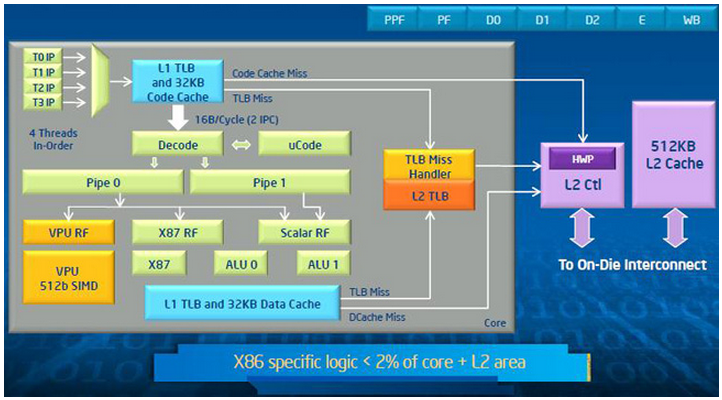
\includegraphics[width=0.7\linewidth]{fig/phi_structure.png}
    \caption{Intel Xeon Phi basic components \cite{intel_phi_architecture}.}
    \label{fig:phi_structure}
\end{figure} 

%%%%%%%%%%%%%%%%%%%%
\subsection{Vector Processing Unit}
The most important part of the MIC core is the VPU\,--\,Vector Processing Unit. VPU contains a new special instructions set of 512 bit SIMD instructions known as Intel Initial Many Core Instructions (Intel IMCI). Thus our VPU can perform 16 operations with a single precision (from here on as SP) and 8 operations with double precision (from here on as DP) in 1 cycle, which by itself sets high performance per core. VPU also supports FMA instructions (Fused Multiply-Add), therefore it can realize 32 SP operations and 16 DP operations at the same time. FMA instructions support multiplication and addition of operands at the same time (FMA is perfect for vector dot product routines).

\par From the energy point of view VPU is a highly developed technology, especially for HPC where the load of the processor's cores is very high. A single operation can perform a lot of work all at once. Without VPU, it would be necessary to repeat certain instructions for each vector component. For the support of 512 bit SIMD instructions, it was necessary to perform various adjustments, like a masking register added into the VPU allowing \uv{per lane predicated execution} (this improved the efficiency of the software pipelining). VPU also supports Gather and Scatter instructions, which allow non-unit stride vector memory access. EMU (Extended Math Unit) can perform transcendent operations like roots, logarithms and other, while optimally using the core's performance.

%%%%%%%%%%%%%%%%%%%%
\subsection{System connection}
As already stated, connection of individual parts within the coprocessor is realized through a two-way circular connection. Each direction is composed of 3 independent rings. The first and the most complex one is the data block ring (BL\,--\,Figure \ref{fig:phi_connection}). Its width of 64 bytes secures support for high throughput, required due to high number of cores. The Address ring (AD\,--\,Figure \ref{fig:phi_connection}) is in contrast simpler and smaller. It serves for sending of memory addresses and read/write commands. The last and the smallest one is the acknowledgment ring (AK\,--\,Figure \ref{fig:phi_connection}), sending the regulation of the flow.

\par If a core is not successful in accessing own L2 cache (L2 miss), the request for the address is sent by the address ring to the tag directories (TD\,--\,Figure \ref{fig:phi_connection}). A Memory addresses are jointly distributed among tag directories to ensure smooth operation on a given ring. If requested data is found in the L2 cache of another core, the request is sent by the address ring to the L2 cache of that core. Subsequently, the data block is sent to the data block ring. If the requested data is not found in any cache, the memory address is sent from the tag directory to the memory bus, and the memory controller serves the request. Memory controllers are symmetrically distributed around the ring which eliminates hotspots and helps to achieve quick response.

\par During a memory access, whenever there is a L2 miss in the core, the core generates a request for an address sent through the address ring (AD) to the tag directory (TD). If the data is not even found in the tag directory, the core generates another request for the address; this time the request is directed to the memory. The memory bus picks up the data block from the memory, and sends it to the core by the data ring (BL). During this process, there are 2 requests for an address, 2 acknowledgment messages (through AK) and 1 data block sent through the ring.

\begin{figure}[htb]
    \centering
    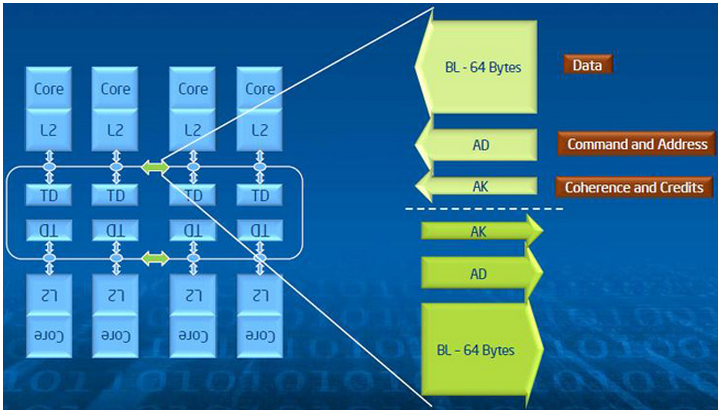
\includegraphics[width=0.7\linewidth]{fig/phi_connection.png}
    \caption{Intel Xeon Phi system connection \cite{intel_phi_architecture}.}
    \label{fig:phi_connection}
\end{figure} 

%%%%%%%%%%%%%%%%%%%%
\subsection{Streaming stores}
Streaming stores are another key enhancement, focused on further improvement of memory throughput. Pseudo code \ref{code_stream_triad}, which demonstrating so called \uv{Streams Triad} is bellow:

\definecolor{lightgray}{gray}{0.93}
\definecolor{solidgray}{gray}{0.25}
\definecolor{oldlace}{rgb}{0.99, 0.96, 0.9}

\lstset{
  language=C,                             % Code langugage
  basicstyle=\footnotesize\ttfamily,      % Code font, Examples:   \footnotesize, \ttfamily
  keywordstyle=\color{blue},              % Keywords font ('*' = uppercase)
  commentstyle=\color{solidgray},         % Comments font
  numbers=left,                           % Line nums position
  numberstyle=\tiny,                      % Line-numbers fonts
  stepnumber=1,                           % Step between two line-numbers
  numbersep=5pt,                          % How far are line-numbers from code
  backgroundcolor=\color{lightgray}, % Choose background color
  frame=none,                             % A frame around the code
  tabsize=2,                              % Default tab size
  captionpos=b,                           % Caption-position = bottom
  breaklines=true,                        % Automatic line breaking?
  breakatwhitespace=false,                % Automatic breaks only at whitespace?
  showspaces=false,                       % Dont make spaces visible
  showtabs=false,                         % Dont make tabls visible
  columns= spaceflexible,                 % Column format
  morekeywords={__global__, __device__},  % CUDA specific keywords
}

\bigskip
\begin{lstlisting}[caption=Streaming Triad example, captionpos=b, label=code_stream_triad]
for(i = 0; i < N; i++)
{
    A[i] = k * B[i] + C[i];
}
\end{lstlisting}
\bigskip

The pseudo code \uv{Stream Triad} reads 2 arrays\,--\,\texttt{B, C} and writes in array \texttt{A}. Historically, the core had had to read cache line before it started to write the addressed data. Therefore, another, needles reading from the memory connected with writing occurs. Streaming store instructions allow the core to write in the memory the entire cache line without the need for reading it from the memory prior to the write. This reduces the number of transferred bytes per 1 iteration from 256\,B to 192\,B. The bottom line is that we never read from \texttt{A} and size of \texttt{A} is bigger than size of L1 cache. In our case when using streaming stores instructions, it is necessary to perform operations: \texttt{Read B, Read C, Write A}. On the contrary without the use of stores streaming instructions it is necessary to perform operations: \texttt{Read A, Read B, Read C, Write A}, which is 1 operation more when compared to the previous case. 

%%%%%%%%%%%%%%%%%%%%
\subsection{Cache memories}
A great amount of effort and attention was spent on the issue of cache memories providing a high throughput. Every core is equipped with a 32\,KB L1 instruction cache, 32\,KB L1 data cache and 512\,KB L2 cache. All cache memories are fully coherent, while they support the x86 memory model. L1 cache memories offer a throughput about 15 times higher than the throughput of the main memory. In comparison with the main memory, the L2 cache is 7 times faster. Because of this, effective use of cache memories is the key factor for achieving peak performance on a MIC. Moreover, working with cache memories is many times more energy efficient than work with the main memory. Therefore, when processing large amounts of data, is very suitable to use \uv{cache-blocking}, which can help to improve cache utilization.

%%%%%%%%%%%%%%%%%%%%
\subsection{Threads}
If we take into account the fact, that the Xeon Phi offers more than 50 cores, while each core disposes with 4 hardware threads, we are getting a fairly decent amount of usable threads. In comparison with the Xeon processor, which uses 8/16 (Hyper-threading off/on) threads at the most, the 200 threads is an astonishing number. Of course, it is not completely simple to effectively use such many threads. Therefore later on, we will talk about procedures which can help us to achieve high performance. As long as our algorithm cannot be scaled for at least 2 threads per core, the application will most likely run ineffectively and even slowly than on a Xeon processor. The use of at least 2 threads per core allows covering performance deficiencies of weaker cores (2 clock cycles instruction decoding), which when compared to the Xeon processor are about 40 times slower (1 Xeon Phi thread vs. 1 Xeon thread). Picture \ref{fig:phi_scaling} depicts the difference of algorithm scaling on the Xeon processor and the Xeon Phi coprocessor. We can observe that the maximum performance can be reached on the Xeon Phi coprocessor only when using at least 2 threads per core. 

\begin{figure}[htb]
    \centering
    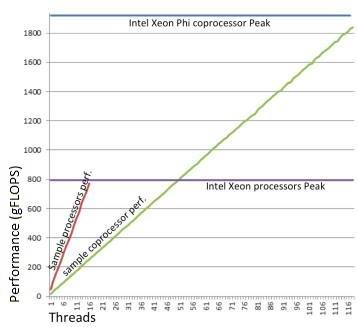
\includegraphics[width=0.7\linewidth]{fig/phi_scaling.jpg}
    \caption{Scaling on threads level (Xeon Phi vs. Xeon) \cite{xeon_phi_book}.}
    \label{fig:phi_scaling}
\end{figure} 

%%%%%%%%%%%%%%%%%%%%%%%%%%%%%%%%%%%%%%%%
\section{Introduction of work station and summary}
All measurements and application development for this thesis were performed on the Anselm supercomputer in Ostrava. Further, basic properties and parameters of the Anselm supercomputer will be presented to give the reader an idea about the machine, which measurements and testing of developed applications were performed on. Anselm is a cluster based on Intel x86-64 nodes built on Bull Extreme Computing bullx technology. The peak performance reaches the level of 94.5 Tflop/s. The cluster contains 4 types of computing nodes \cite{anselm_guide}:

\begin{enumerate}
\item{Computing nodes without accelerator\,--\,180 nodes}
\item{Computing nodes of the Fat type\,--\,2 nodes}
\item{Computing nodes with a GPU accelerator\,--\,23 nodes}
\item{Computing nodes with a MIC accelerator\,--\,4 nodes (for this thesis the most important ones):
    \begin{itemize}
    \item{64 processor cores total (38.4\,gFLOPS per core for SP data)}
    \item{2x Intel Sandy Bridge E5-2470, 8 core, 2.3\,GHz processor for each node}
    \item{1x MIC accelerator Intel Xeon Phi 5110P per node}
    \item{bullx B510 blade servers}
    \item{memory organization:
        \begin{itemize}
        \item{2 sockets per node}
        \item{data transfer speed up to 1600\,MT/s}
        \item{memory controllers are integrated in the processor}
        \item{6x DDR3 DIMMS per node}
        \item{3x DDR3 DIMMS per processor (38.4\,GB/s)}
        \item{1x DDR3 DIMMS per channel}
        \end{itemize}
    }

    \end{itemize}
}
\end{enumerate}

%%%%%%%%%%%%%%%%%%%%
\subsection{Detailed specification of the Intel Xeon Phi coprocessor}
\begin{itemize}
\item{Pentium scalar ISA including x87 \cite{xeon_phi_book}}
\item{AVX-512 (extended instruction set)}
\item{In-order operations, super-scalar issue}
\item{Full 64 bit addressing}
\item{4 hardware threads per core}
\item{50 to 61 cores (in our case 60 cores)}
\item{2 cycle decoder}
\item{Scalar and vector unit}
\item{2x pipeline (scalar and vector/scalar) 
\item{6-16\,GB GDDR5}
\item{320\,GB/s}
\item{Peak performance 2\,tFLOPS for SP data}
}
\item{L1 cache:
    \begin{itemize}
    \item{32\,B instruction cache per core}
    \item{32\,KB data cache per core}
    \item{8 way associative}
    \item{64\,B cache line}
    \item{3 cycle latency}
    \item{up to 8 unresolved requests}
    \item{Fully coherent }
    \end{itemize}
}
\item{L2 cache:
    \begin{itemize}
    \item{512\,KB per core}
    \item{8 way associative}
    \item{64\,B cache line}
    \item{11 cycle latency}
    \item{Inclusive}
    \item{Up to 32 unresolved requests}
    \item{Streaming HW prefetcher}
    \item{Fully coherent}
    \end{itemize}
}
\end{itemize}

%%%%%%%%%%%%%%%%%%%%%%%%%%%%%%%%%%%%%%%%%%%%%%%%%%%%%%%%%%%%%%%%%%%%%%%%%%%%%%%
\chapter{Process for algorithm implementation}

%%%%%%%%%%%%%%%%%%%%%%%%%%%%%%%%%%%%%%%%
\section{Platform selection}
At the beginning we should clarify when is it suitable for application to use a CPU and when a MIC. Therefore we summarize \ref{tab:table_comparasion_features} the most significant differences. This chapter is based on information from \cite{xeon_phi_book}, \cite{intel_phi_architecture}, \cite{intel_compiler_pragmas} and \cite{openmp}.

\begin{table}[ht]
\catcode`\-=12
\begin{center}
\begin{tabular}{| l | r |} \hline
{\large \textbf{Intel Xeon processor (CPU):}} & \large{\textbf{Intel Xeon Phi coprocessor (MIC):}}\\ \hline
High performance of single thread & High level parallel processing\\ \hline
High capacity memory & High throughput memory\\ \hline
8 cores & Up to 61 cores (in our case 60)\\ \hline
2 hardware threads per core & 4 hardware threads per core\\ \hline
Hyperthreading: Yes (but now always used) & Hyperthreading: Yes\\ \hline
SIMD instructions (256 bit registers) & SIMD instructions (512 bit registers)\\ \hline
Intel AVX & Intel AVX-512\\ \hline
Virtualization, AES & Gather/scatter instructions, FMA\\ \hline
Intel 307/614\,gFLOPS (8/16 threads, SP) & 2000\,gFLOPS (SP)\\ \hline
38,4\,GB/s & 320\,GB/s\\ \hline

\end{tabular}
\caption{Comparison of a features of the CPU and the MIC.}
\label{tab:table_comparasion_features}
\end{center}
\end{table}

Differences in the architecture of the CPU and MIC definitely aren't negligible. And it is necessary to consider them when selecting a platform for running an application and for writing the application itself. As long as our application is not optimized sufficiently, it is not suitable to use a MIC, it is better to choose a CPU. The CPU is designed in a way that allows for sufficient performance even when running a not optimized application on single thread. On the contrary running an application, which is not vectorized and sufficiently parallelized for a MIC, we are left with results orders of magnitude worse than on a processor. Decision making process for selection of suitable platform can be seen in the picture \ref{fig:platform_selection}.

\begin{figure}[htb]
    \centering
    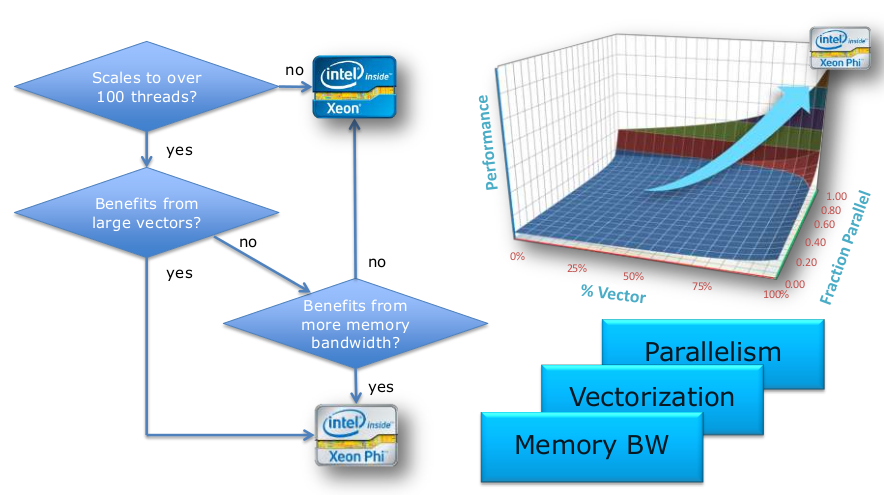
\includegraphics[width=0.7\linewidth]{fig/platform_selection.png}
    \caption{Process for platform selection \cite{xeon_phi_book}.}
    \label{fig:platform_selection}
\end{figure} 

When choosing the platform it is therefore necessary to consider: the possibility of using a large number of threads, the possibility of vectorization and the possibility to use high throughput memory. Based on the above picture we start the decision making process with number of usable threads. If our application can use more than 100 threads (of course 100 threads is not precisely set value, it depends on specific application), a MIC can seem like a good choice. However, if our application is not capable to use this number of threads, it is better to use the processor instead.

\par If our program can also profit from wide vectors (512 bit AVX registers for Xeon Phi), the coprocessor will be the correct choice. Of course, everything depends on the optimization of the algorithm, which is the key aspect of performance.

\par If we are not capable to vectorize the code sufficiently, the Intel Xeon Phi coprocessor is providing us with the possibility to use high throughput memory, e.g. for processing of a large data (through high number of threads). If we are not able to use even this option, we use the Xeon processor to run the application. 

%%%%%%%%%%%%%%%%%%%%%%%%%%%%%%%%%%%%%%%%
\section{Optimization process}

%%%%%%%%%%%%%%%%%%%%
\subsection{Introduction to optimization}
It is suitable and recommended to optimize the application for the CPU first. After reaching high level of optimization especially if our application is capable of using a high number of threads, we can move to the MIC platform. When developing applications for this platform it is necessary (for now) to use an Intel compiler (\texttt{icc, icpc, ifort}) to generate code for the MIC architecture. Furthermore the compiler automatically trying to optimize the code (if the optimization is not explicitly turned off). However, this is not always possible, especially due to naive algorithms, which are not optimized. Frequent reasons are jumps and branching, which are constantly repeated in every iteration, embedded loops, poor work with memory or simply incorrectly chosen algorithm structure. With a great number of iterations, a single condition that the program has to evaluate in every iteration can unbelievable slow down the program. Furthermore this loop cannot be unrolled and vectorized. Similarly it is more than suitable to eliminate the number of accesses to the main memory, which results in the processor waiting for the data a number of cycles more than reading the data from the cache memory.

\par Removal of needless and frequently repeated jumps in the algorithm and enhancement of reading the data from the cache memory can bring us significantly higher performance. However, it is possible that the code modified in this way will not be \uv{appealing} from a programmer point of view, it will not be readable and transparent, which we are trying to have most of the time. It is price paid for achieving the maximum performance. Sometimes, it is necessary to use such constructs which make the code intricate but the compiler can optimize them better and thus generate a significantly faster code.

\par However, automatic optimizations of the compiler do not have to be sufficient, therefore there are several ways how to help the optimization. Later on we will deal especially with compiler directives like \uv{Intel \#pragma} or \uv{OpenMP \#pragma}, which are special marks for compiler, thank to which it can optimize the code in a better (worse) way. These directives are placed usually above the loops we are trying to optimize. Thanks to these special designations we know e.g. how to signal the compiler that it can (or even has to) vectorize a given section of the code, start it on several threads, mark that a given data is aligned in the memory, etc. All of these compiler options can only be used if we precisely know their meaning and consequences of use, otherwise many issues might occur bad computing results or even an unexpected crash of the program. Thats why the meaning of individual directives (of course only a few significant ones, others can be found directly in the compiler documentation \footnote{\url{https://software.intel.com/en-us/compiler_15.0_ug_c}}, some Intel guides \footnote{\url{https://software.intel.com/en-us/articles/getting-started-with-intel-composer-xe-2013-compiler-pragmas-and-directives}}, etc.) will be explained and demonstrated on prime examples.

\par For peak performance the most important optimization steps are: vectorization, exploiting the cache memory and running the program on many threads. Vectorization is extremely important especially because the CPU/MIC can employ VPU to treat vectors instead of scalar operations. The exploiting of the cache memories can be enhanced by keeping the working data in cache as along as possible and not move it needlessly between the main memory and on-chip memory. Another important thing is the parallelization of the algorithm on the thread level. Under this term we mean splitting the computing (if it is possible) among several threads. Each hardware thread computes results for its own data block, which in the end make up for the final result. At every step of the optimization, it is necessary to consider a large number of factors affecting the end speed of the program. Since there's no silver bullet, one must experiment. Detailed process of optimization will be outlined in subsequent chapters.

\par If we have reached the state when our code is sufficiently vectorized, parallel and we believe we cannot enhance the CPU's performance anymore, it is time to move to the MIC. Unlike 8/16 hardware threads offered by the CPU, the MIC offers more than 200 hardware threads. It is here where we find the possibility how to very quickly and simply try to accelerate the computing on the MIC when compared to the CPU. Therefore it is advisable to experiment with various numbers of threads, e.g. 60, 120, 180 and 240 threads. In theory, it should be that by doubling the number of threads the computing time shortens to half. However the reality is frequently different, it depends on the type of algorithm and level of optimization (and overhead caused by threads communication).

\par In order to make such a large number of threads sensible, it is necessary to secure that all the threads have enough work to do, otherwise overhead can slow down the program. Thus, the size of processed data is another important factor for selection of the suitable platform. If the computing time is better when compared to the CPU, we are on the right way to exploit the potential of the MIC, however the algorithm can be probably still modified and improved to achieve higher performance.

\par Application which was optimal for the CPU does not have to be optimal for our coprocessor due to different architecture. For example, the MIC when compared to the processor has a higher memory throughput, bigger L2 cache, enhanced instruction set, etc. Thus, if we want to get maximum out of the MIC, it is necessary to consider all the aspects and modify the code based on its needs. 

%%%%%%%%%%%%%%%%%%%%
\subsection{Vectorization}
Simply told, vectorization is a transformation of scalar operations to vector operations. Scalar operations work with 1 pair of operands. While vector operations can process many more pairs of operands at the same time.Vectorization is realized by the compiler (and user) by packing a sequence of scalar operations into a vector one. During vectorization 512\,bit SIMD (Single Precision Multiple Data) instructions are generated. In our case the processing of SIMD instruction is secured by the VPU unit, which as we already stated can process 512 bit vectors of operands.

\par The Intel compiler can automatically vectorize sample codes (as long as optimizations aren't explicitly prohibited) based on certain heuristics. Automatic optimization are executed only if the compiler is sure that the vectorization of the code won't change its semantics (e.g. during mutual data dependency of processed vector elements). In the cases when the compiler refuses to vectorize the code (and we are certain that vectorization won't affect the semantics of the code), it is possible to override standard behavior by compiler directives like \texttt{\#pragma ivdep, \#pragma simd}. The meaning of individual directives will be explained later.

%%%%%%%%%%%%%%%%%%%%
\subsection{Memory layout}
During algorithm optimization a good storage of data in memory is extremely important. If we have decided to store data in structures, we usually have 2 options available\,--\, array of structures (AoS) and Structure of arrays (SoA). First way (AoS) can have the following form:

\bigskip
\begin{lstlisting}[caption=Array of structures example, captionpos=b, label=AoS]
struct
{
    float x;
    float y;
    float z;
} AoS[N];
\end{lstlisting}
\bigskip

If we consider general data storage in array we discover that individual components of the array are stored continuously in memory. In this case, we will have an array of structures stored in memory containing items \texttt{x, y, z}. This trinity represents one structure, i.e. one element of the array. Next element of the array will be another structure etc. Between individual elements of the array there can be a certain padding, which serves for better alignment of data in the memory. The downside of this solution is especially that if our algorithm wants to read/write from/to all elements (structures) for example component \texttt{x}, it is not possible to use simple and quick read/write vector instructions, but gather/scatter instructions. These instructions allow non-unit stride memory access. Under these circumstances the compiler won't vectorize the code, thus we loose performance. Moreover, the gather/scatter instructions require more CPU cycles than simple load/store instructions. To make data SIMD-friendly, structure of arrays (SoA) will be better way:

\bigskip
\begin{lstlisting}[caption=Structure of arrays example, captionpos=b, label=SoA]
struct
{
    float x[N];
    float y[N];
    float z[N];
} SoA;
\end{lstlisting}
\bigskip

\par Data stored in a SoA is in this case more preferable solution because it eliminates the need of gather/scatter instructions. In this case, we have arrays \texttt{x, y, z} stored continuously in the memory. These 3 arrays together make up one structure. If our algorithm repeatedly accesses neighbors elements of array \texttt{x} (unit stride), the compiler can generate vector read/write instructions. Prefetching of data to cache memory works also better while we can maximally use their size. This solution is more suitable also in regards to the alignment of data in memory because it is sufficient to align the whole arrays once (not every array component as was the case with AoS). Thus the paddings don't occupy memory space.

%%%%%%%%%%%%%%%%%%%%
\subsection{Directive \texttt{ivdep/IVDEP}}
The directive ivdep/IVDEP instructs the compiler to ignore expected data (vector) dependencies in \texttt{for} loops. Implicitly, the compiler treats expected data dependencies as proved data dependencies. This is conditioned by the fact that if the compiler doesn't have a confirmed data independency in a given loop, it will not execute vectorization due to the possibility of unexpected behavior of the program. The use of \texttt{ivdep} directive is therefore suitable only in case when we are sure that expected data dependencies do not apply and the code can be vectorized safely. If the data dependency is confirmed, the compiler simply ignores the \texttt{ivdep} directive.

%%%%%%%%%%%%%%%%%%%%
\subsection{Directive \texttt{simd/SIMD}}
The simd directives serves just like the ivdep directive for sending an instruction to the compiler to vectorize the processed section of the code (internal loop). As opposed to the \texttt{ivdep} directive, there is one significant difference. Pragma \texttt{simd} instructs the compiler to always vectorize the cycle located under this directive. All data dependencies including the confirmed ones are ignored, the heuristic of the compiler is completely changed, loop is vectorized irrelevantly on the possibility of negative consequences on the the application. With incorrect use computational errors or other unexpected behavior might occur. Pragma \texttt{simd} is a powerful tool giving the programmer full control over the vectorization possibilities.

%%%%%%%%%%%%%%%%%%%%
\subsection{Directive \texttt{vector aligned/VECTOR ALIGNED}}
When using this directive, we again instruct the compiler that it can ignore its optimal heuristics, this time regarding the data alignment in memory. But in order to use the vector aligned directive, we have to store the data (arrays) in memory at aligned addresses. For this purposes a \texttt{\_mm\_malloc(int size, int align)} function can be used. It aligns the data in memory for multiples of the \texttt{align} parameter. By using the \texttt{vector aligned} directive the compiler can generate instructions for moving aligned arrays, thus the runtime alignment control does not have to be performed. Conversely, unaligned data forcing compiler to generate gather/scatter instruction. Again, one must be extra careful when using the \texttt{vector aligned} directive and use it only if we are certain that data is aligned. Otherwise the code will crash.

%%%%%%%%%%%%%%%%%%%%
\label{sec:omp_parallel}
\subsection{Directive \texttt{omp parallel}}
Pragma \texttt{omp parallel} explicitly authorizes the compiler for parallelization of selected section of the code. The directive is part of the \texttt{OpenMP} library. The directive creates a logic group of threads (executing the same code), the number of which can be set by changing the environment variable (\texttt{export OMP\_NUM\_THREADS=N}) or directly in the source code by using the function \texttt{omp\_set\_num\_threads} (for C and C++ languages). For the MIC it is possible to create and use in this way more than 200 threads that works really in parallel.

%%%%%%%%%%%%%%%%%%%%
\label{sec:omp_for}
\subsection{Directive \texttt{omp for}}
The \texttt{omp for} directive authorizes the compiler for distribution of individual loop iterations among a logic group of threads created by on \texttt{omp parallel} directive. The directive has to be placed in the code immediately before the \texttt{for} loop. It is important to consider and correctly determine which variables will be shared among the threads and which will be private for each threads. Before parallelization of the cycle it is necessary to secure that individual iterations will be independent, otherwise incorrect results occur and the computation slows down. It is necessary for the iteration variable to be private for each thread. The iteration variable cannot be changed in the body of the loop; the loop can only have one entry point, one exit point and it cannot contains \break{break} command (or any other jump command). There are lot of clauses\footnote{List of clauses associated with \texttt{omp for} directive can be found on page
\url{https://computing.llnl.gov/tutorials/openMP/}} associated with \texttt{omp for} directive which can influence threads behavior. It is used e.g. for threads \texttt{scheduling}, synchronization (\texttt{barrier}), \texttt{reduction} etc.

%%%%%%%%%%%%%%%%%%%%
\subsection{Memory allocation}
\label{sec:allocation}
For dynamic allocation of aligned memory block \texttt{\_mm\_malloc(int size, int align)} function can be used. The \texttt{size} parameter indicates memory size (in Bytes). Data is aligned in the memory to multiples of the \texttt{align} parameter. For the Intel Xeon Phi coprocessors it is suitable to align the data to multiples of 64\,Bytes (64\,Bytes cache line).

\par To release of dynamically allocated memory (with the \texttt{\_mm\_malloc} function) it is necessary to use the \texttt{\_mm\_free} function. When using the standard function \texttt{free(void *p)} we risk unexpected program behavior.

%%%%%%%%%%%%%%%%%%%%
\subsection{Binding of threads}
\texttt{KMP\_AFFINITY} is an environment variable that determines the placement of threads across the CPU or MIC cores. We can use 2 basic types of threads affinity\,--\,\texttt{scatter} and \texttt{compact.} The scatter affinity determines that threads are evenly distributed over cores of the CPU/MIC. So if we want to use 120 threads on a MIC, and set the threads affinity to \texttt{scatter}, each core of the MIC will obtain 2 threads to run. Therefore, the load will be evenly distributed between all cores. On the other hand if we set the threads affinity to \texttt{compact}, each core will run the maximum number of threads (4 in our case), thus we fully use 30 cores while other 30 are idle. Which threads distribution is more suitable depends on specific algorithm, quantity of processed data, etc.

%%%%%%%%%%%%%%%%%%%%
\subsection{NUMA First Touch Policy}
The NUMA abbreviation means Non-Uniform Memory Access. It is a technology used in modern systems for faster access of the processor to memory. The processor works with memory integrated directly on the chip (On-chip memory) or memory, which is connected to the processor through bus (Off-chip memory). For example our Xeon Phi coprocessor has its own L1 and L2 cache on each core, while it is connected to the main memory through PCIe bus. The issue is that each core (or thread) can have access to given section of the memory of different complexity. Therefore it is suitable for the data to be distributed in the memory in such a way, that each thread will have data stored in the memory as close as possible to given core.

\par This case can be achieved by the method called \uv{NUMA First Touch Policy}. In this case we use the fact that the memory is physically occupied only at the moment of its primary initialization. Therefore, the primary initialization of the memory has to be executed in parallel by all the threads. By this we will achieve that every thread will place its data into a memory where they have best access. During the primary memory initialization by a single thread all the data would be placed in a way where other threads could have slower access.

%%%%%%%%%%%%%%%%%%%%%%%%%%%%%%%%%%%%%%%%
\section{Programming models}
Programing models are in this case different approaches to creation of application (in terms of MIC utilization during program runtime). We distinguish 2 basic models (discussed in this thesis)\,--\,native and offload. Another interesting model is also cluster mode (when we use more MICs at once).

%%%%%%%%%%%%%%%%%%%%
\subsection{Native mode}
It is suitable to use the native mode only for programs made mostly of operations which can be parallelized either by vectors or threads (both in best case). These programs should not execute a greater number of I/O operations; MIC cannot handle them as good as the host system. It is not suitable for programs containing significant sections of the code processed sequentially.

\par Creating a native application for a MIC isn't difficult. Source code written in C, C++ or Fortran languages and Intel compiler is sufficient. This code then needs to be compiled with the \texttt{-mmic} parameter, specifying that this is a program created for the MIC architecture. After successful compilation, the program is ready for execution. Since it's a native program, it is necessary to be logged in on specific MIC card via \texttt{ssh}. We should set necessary environment variables and execute the program. If the host system doesn't share the file system with the coprocessor, it is necessary to manually copy the executable file, libraries and other important  files over. The \texttt{scp} utility serves for this purpose. Advantages of the native mode are simpler implementation and the resulting speed of the program. Of course the resulting speed of the program depends on a number of factors, so it is suitable to use it only under certain conditions. 

%%%%%%%%%%%%%%%%%%%%
\subsection{Offload mode}
The offload modes primarily uses CPU to run the application, however some parts of the program run on a MIC. It's a more complex solution than the native mode, its implementation is slightly more difficult. This mode is very similar to GPGPU programing (we can use also OpenCV). The program itself is developed and executed on the host system while some computation parts are offloaded to the MIC. Offload applications are suitable in cases when a program executes a great number of I/O operations (generally operations performed sequentially), while it contains computationally demanding sections which can be processed in parallel. Sequential operations are computed by the host system and parallel sections will be processed on the MIC (using a great number of threads). There are two basic types of offload mode.

\par \textbf{Model without a shared virtual memory} is more demanding on the implementation but allows the programmer full control over the data transfers between CPU and MIC. After launch, the program is executed on the CPU until the \texttt{\#pragma offload} \footnote{List of clauses associated with offload directive can be found on page
\url{https://software.intel.com/en-us/articles/xeon-phi-coprocessor-data-transfer-array-of-pointers-using-language-extensions-for-offload}} directive is encountered (this is an Intel compiler directive, OMP directives can be used as well, e.g. \texttt{\#pragma omp target}). This directive causes that the compiler and runtime library will perform a data transfer (the programmer could decide what exactly will be transferred) between the CPU and the MIC, execution of the program on MIC, eventual data transfer back from the MIC to the CPU. Only scalar data types, arrays and structures can be transferred (types which can be copied by the \texttt{memcpy} function). If we want to work in the offload mode with more complex data types or dynamic structures, we have to use a model with shared virtual memory. CPU and MIC can execute code in parallel, of course with limitation when waiting for various data. This offload mode is supported by the C, C++ and Fortran languages. Data transfer between host and coprocessor has to be explicitly solved by the programmer; the compiler is not able to do it on its own.

\par Parts of the code (function), which we want to execute on the coprocessor in offload mode has to be added an attribute during its definition (declaration). It tells the compiler that this code is designed for the MIC architecture. This can be done e.g. by \texttt{\_\_attribute\_\_((target(mic))).}
Declaration of the function designed for offload mode can have this form:

\bigskip
%\begin{lstlisting}[caption=Declaration of offload function, captionpos=b label=code_offload_declaration]
\texttt{\_\_attribute\_\_((target(mic))) void offload\_function(void);}
%\end{lstlisting}
\bigskip

Pseudo code example of offlad usage:

\bigskip
\begin{lstlisting}[caption=Example of offload mode usage, captionpos=b, label=code_offload_usage]
// code running on the processor
processor_function();
#pragma offload target(mic)
{
    // code running on the coprocessor
    offload_function();
 }
// code running on the processor
processor_function();
\end{lstlisting}
\bigskip

The model with \textbf{shared virtual memory} relates to the extension of the C++\,--\,\uv{Intel Cilk Plus language}. For offload mode \texttt{\_Cilk\_shared} and \texttt{\_Cilk\_offload} keywords are used. The offload model with the use of Intel Cilk Plus language does not have support for the Fortran. Variables, we want to share between CPU and MIC are marked specially by the key word \texttt{\_Cilk\_shared.} These variables can then be used on the CPU as well as the MIC. For dynamic memory allocation \texttt{\_Offload\_shared\_malloc, \_Offload\_shared\_aligned\_malloc, \_Offload\_shared\_free} and \texttt{\_Offload\_shared\_aligned\_free} are used.

\par As stated, this mode allows transferring more complex data types like dynamic structures, objects, pointers, etc. Work in this offload mode is simpler; the programmer is not dealing with data transfer between CPU and MIC as much as is the case without shared virtual memory.

\par Apart from previous two offload models, also the \textbf{Auto Offloading} mode can be used. This mode can be used with routines of the Intel MKL library. If our program uses a MKL function and processes sufficient a quantity of data, the computation can be automatically moved to the MIC. After computation on the coprocessor, the result is returned to the host system. To achieve the automatic offload, we have to enable it e.g. by setting environment variable \texttt{MKL\_MIC\_ENABLE=1}). We will discuss this process in more detail in a practical example.

%%%%%%%%%%%%%%%%%%%%%%%%%%%%%%%%%%%%%%%%
\section{Performance measurement}

%%%%%%%%%%%%%%%%%%%%
\subsection{Time measurement} 
Time measurement of computing can be realized in many way. E.g. calling of the \texttt{gettimeofday} (library \texttt{sys/time.h}) function can be used before beginning the computation and after the computation, while the results are stored in the \texttt{timeval} structure. The resulting times have to be simply subtracted from one another to get final time. Even simpler is to use the function \texttt{omp\_get\_wtime} (library \texttt{omp.h}), also before beginning the computation and after its completion. However, if we want to know as much as possible about the performance of our application, time measurement is not sufficient on its own. Because of this it is suitable to use a more powerful tool, which could provide us accurate information about the operation of our program. For this purpose we decided to use the \texttt{PAPI} library.

%%%%%%%%%%%%%%%%%%%%
\subsection{PAPI}
The PAPI library \footnote{The PAPI library is available together with the documentation on page \url{http://icl.cs.utk.edu/papi/}} provides a development tool with simple interface for work with hardware counters on majority of microprocessors. The PAPI library allows the programmer almost in real time to see dependencies between the performance of developed software and processor events. PAPI provides access to a collection of components, which allow for performance measurement and possibilities across hardware and the program itself.

\par After installing the PAPI library, by using the \texttt{papi\_avail} (or \texttt{papi\_native\_avail}) command one can find out which hardware counters are available. In this project, the following PAPI options have been used.

\begin{itemize}
\item{\texttt{PAPI\_FP\_OPS}\,--\,Floating point operations per second}
\item{\texttt{PAPI\_SP\_OPS}\,--\,Vector (floating point) operations per second}
\item{\texttt{perf::L1-DCACHE-LOADS}\,--\,L1 data cache loads}
\item{\texttt{perf::L1-DCACHE-STORES}\,--\,L1 data cache stores}
\item{\texttt{PAPI\_L1\_DCM}\,--\,L1 data cache misses}
\item{\texttt{PAPI\_L2\_DCA}\,--\,L2 data cache accesses}
\item{\texttt{PAPI\_L2\_DCM}\,--\,L2 data cache misses}

\end{itemize}

PAPI has a very good support for Xeon processors. Unfortunately, at the time of creation of this thesis it had only a limited support for Xeon Phi coprocessors. E.g. the support for number of FP vector operations was missing, which is a significant indicator for program optimization.  
However, if we develop application for CPU and MIC at the same time, it is sufficient to measure performance and computation time on the CPU and computation time on the MIC. Based on the computation time on the MIC it is then very simple to calculate reached performance in comparison with the CPU.
If we want to get really detailed information about our application, the most suitable solution is to use a powerful tool directly from Intel - VTune Amplifier. This tool collects information during the operation of the program, which is then displayed in graphic form.

%%%%%%%%%%%%%%%%%%%%%%%%%%%%%%%%%%%%%%%%%%%%%%%%%%%%%%%%%%%%%%%%%%%%%%%%%%%%%%%
\chapter{Intel Xeon Phi in practice}
So far we have been dealing mostly with theory in the field of architecture and implementation of algorithms on the MIC. Now, the time has come to move from theory to practice. In the following subchapters we will describe two exemplary tasks, implemented in this thesis. We will begin with a well know benchmark, which is a matrix vector multiplication. Later, we will describe a more complex algorithm representing simulation of particles system (N-Body). Both applications are implemented with the purpose of achieving the highest performance of the MIC (we will going to expertise and experience). After solving these examples, we will focus on much more complicated problems such as optimization of k-Wave simulations or cross-compilation of some existing programs and libraries.

%%%%%%%%%%%%%%%%%%%%%%%%%%%%%%%%%%%%%%%%
\section{Matrix vector multiplication (matvec)}

%%%%%%%%%%%%%%%%%%%%
\subsection{Introduction of the benchmark}
\label{sec:matvec_intro}
This is essentially a simple algorithm, which can be described by a pseudo code, as follows:

\bigskip
\begin{lstlisting}[caption=Matrix vector multiplication pseudo code., captionpos=b, label=code_matvec]
for(i = 0; i < ROWS; i++)
{
    for(j = 0; j < COLS; j++)
    {
        vector_final[i] += matrix[i][j] * vector[j];
    }
}
\end{lstlisting}
\bigskip


The result of matrix vector multiplication is therefore a vector. Every elements (of final vector) are a dot product of one matrix row and input vector. At first sight the algorithm appears to be simple (is true) but we cannot call it an optimal implementation capable of exploiting the performance of the CPU/MIC. The following pars describe how to proceed with optimization of this algorithm. First, I will remind that during the creation of this thesis the Intel C++ compiler was exclusively used (\texttt{icpc}). Therefore, all possibilities and options of the compiler mentioned apply to the Intel compiler and do not have to be compatible with other compilers. Significance of some used compiler options will by described, but for deeper understanding it is good to go over the documentation\footnote{\url{https://software.intel.com/en-us/compiler_15.0_ug_c}}.

%%%%%%%%%%%%%%%%%%%%
\subsection{Naive implementation}
The naive implementation in C++ language is stems from the pseudo code \ref{code_matvec}. Individual vectors are allocated statically on the stack. The matrix is represented by a 2 dimensional array also allocated statically on the stack. The arrays are not aligned in the memory, optimizations of the compiler are deactivated by the means of the \texttt{-O0} switch (implicitly \texttt{-O2}) (wen are using no vectorization and no parallelism). The compilation of the program can be done as follows:

\bigskip
\begin{lstlisting}[caption=The compilation for CPU and MIC., captionpos=b, label=code_compilation, language=bash]
[host]$ icpc -O0 matvec.cpp -o matvec-host # for CPU
[host]$ icpc -mmic -O0 matvec.cpp -o matvec-mic # for MIC
\end{lstlisting}
\bigskip

After compilation, we get an executable file. After execution we can check the result of the computation and the program's running time.

\par In order to analyze the performance, it is necessary to create a more complex project to simpler work with source codes. For purposes of this thesis the \texttt{matvec/} directory has been created (everything is located in the Appendix \ref{appendix}, next we will identify each step of optimization only by directory name). The project was managed by the means of the \texttt{Gitlab} system (hosted on the school server \texttt{http://pcjaros-gpu.fit.vutbr.cz/}). All source codes are also available at the Bitbucket \url{https://bitbucket.org/xsimek23/intel-xeon-phi-bachelor-thesis}.

\par The \texttt{matvec/naive} directory contains naive implementation of the algorithm described in the benchmark introduction \ref{sec:matvec_intro}. Compilation of the source files (\texttt{make}) is followed by the execution of the program (\texttt{make run}) for the matrix size 64*64 items (on CPU). We decided to use single precision for matrix and vector data. We are working with matrix size of 16\,KB and 2 vectors, each of 256\,B big. We set the repetition of computation at e.g. 1000000.

\par The application is compiled and executed on the CPU. Under these conditions, the computation time is 14.85 seconds and performance is only 593.5\,mFLOPS (floating point operations per second). This is about 1.5\% of total core performance. We can see (Table \ref{tab:table_matvec_naive}) that number of vector and scalar operations are the same. It is because the compiler generate SSE/AVX instruction, but uses only single vector line (scalar operations) while other lines are masked.

\begin{table}[ht]
\catcode`\-=12
\begin{center}
\begin{tabular}{| l | r | r |} \hline
\textbf{Matrix Size (items)} & 64x64 & 128x128\\ \hline
\textbf{Wall Time (s)} & 14.85 & 59.89\\ \hline
\textbf{Scalar FP Operations (mFLOPS)} & 593.5 & 607.1\\ \hline
\textbf{Vector FP Operations (mFLOPS)} & 593.5 (1.5\%) & 607.1 (1.6\%)\\ \hline
\textbf{L1 miss} & 0\% & 1\%\\ \hline
\textbf{L2 miss} & 0\% & 0\%\\ \hline
\end{tabular}
\caption{Performance measurement of naive implementation, compiler options disabled (CPU).}
\label{tab:table_matvec_naive}
\end{center}
\end{table}

By using the \texttt{-optreport} and \texttt{-vec-report3} options, the compiler provides us information about program optimizations. It is e.g. information about what loops were vectorized, unrolled, etc. Based on the compiler information we know that the nested loop could not be vectorized. Therefore, we will have the opportunity to take certain steps leading to successful vectorization.

%%%%%%%%%%%%%%%%%%%%
\subsection{Automatic optimizations, vectorization, padding}
The first choice is to enable automatic optimizations by the \texttt{-O2}, or the \texttt{-O3} option. Further, we tell the compiler that we want to use (if possible) the AVX instruction set. We do this by \texttt{-xavx} (\texttt{OPTFLAGS=-O3 -xavx}) switch. After compilation of the program we discover that the internal loop cannot be vectorized due to presumed data dependences of the vectors. However, in our case there are no real data dependencies, therefore we submit this information to the compiler, e.g. by using the \texttt{IVDEP} directive. Adjusted pseudo code can look like this:

\bigskip
\begin{lstlisting}[caption={Matrix and vector multiplication pseudo code, IVDEP directive.}, captionpos=b, label=code_matvec_ivdep]
for(i = 0; i < ROWS; i++)
{
    #pragma ivdep
    for(j = 0; j < COLS; j++)
    {    
        vector_final[i] += matrix[i][j] * vector[j];
    }
}
\end{lstlisting}
\bigskip

Another important feature is a nice matrix size. Pretty good matrix sizes are multiples of 16. If we had a matrix of size e.g. 63*63, the performance  decreases due to bad memory alignment. For better memory alignment we have to add some padding (during initialization of matrix and vector), which fills empty elements in the matrix (then we will have matrix of size 64*64). After compilation and execution we are able to achieve results:

\begin{table}[ht]
\catcode`\-=12
\begin{center}
\begin{tabular}{| l | r | r |} \hline
\textbf{Matrix Size (items)} & 64x64 & 128x128\\ \hline
\textbf{Wall Time (s)} & 0.66 & 2.87\\ \hline
\textbf{Scalar FP Operations (mFLOPS)} & 96.9 & 48.3\\ \hline
\textbf{Vector FP Operations (mFLOPS)} & 13841.5 (36\%) & 13250.5 (35\%)\\ \hline
\textbf{L1 miss} & 0\% & 22\%\\ \hline
\textbf{L2 miss} & 0\% & 0\%\\ \hline
\end{tabular}
\caption{Performance measurement of vectorized implementation, compiler options enabled, xavx (CPU).}
\label{tab:table_matvec_vec_padding}
\end{center}
\end{table}

From table \ref{tab:table_matvec_vec_padding}, we can see significant improvement. The computation speed increased more than 20 times, the number of vector operations executed per second too. In this case, we achieved 35\% of core performance. If we use matrix of size 128*128, performance will slightly slow down. It is cause by bigger size of the matrix (64\,KB), which is 2 time bigger than L1 cache (data are located in L2 cache). However, we still cannot be satisfied because there are still more steps, through which further increase of performance could be achieved. We can also see importance of padding (data alignment) in the Figure \ref{fig:graph_matvec_padding_exp}. Depending on the data size, we can achieve more than two-fold increase of performance (due to better memory alignment). Source files of this step can be found in the directory \texttt{matvec/vec-padding}.

\begin{figure}[htb]
    \centering
    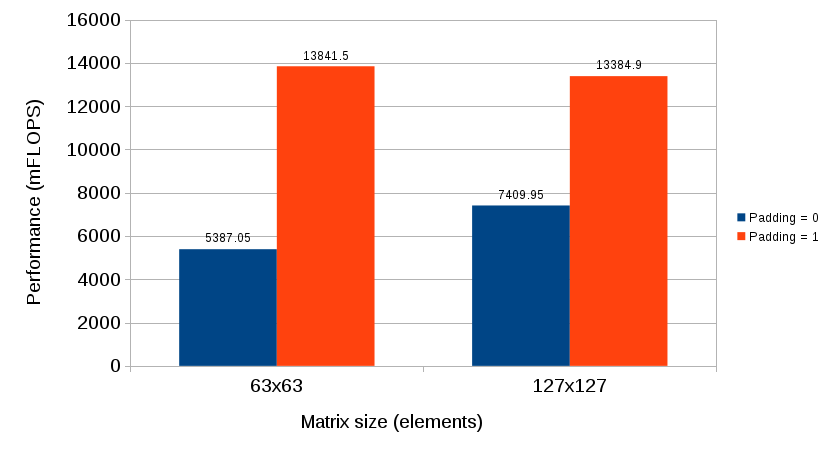
\includegraphics[width=1\linewidth]{fig/matvec_padding_experiment.png}
    \caption{Padding experimets (CPU).}
    \label{fig:graph_matvec_padding_exp}
\end{figure}

%%%%%%%%%%%%%%%%%%%%
\subsection{Dynamic allocation, data alignment}
Another very important step of optimization will be storing the data in the memory. We begin by allocating the data dynamically. This is necessary due to a large quantity of data will be used for future tasks. Under normal condition we would use \texttt{malloc} for dynamic memory allocation on the heap. However, we demand the data to be aligned in the memory (\texttt{\_mm\_malloc}and \texttt{\_mm\_free}, see Section \ref{sec:allocation}). For CPU it is suitable to align the data to 32\,Bytes, for MIC 64\,Bytes. However, we can use a uniform alignment to 64\,Bytes. When the vectors in the memory are aligned, we have to inform the compiler about that. We can use e.g. the \texttt{VECTOR ALIGNED} directive. After adjustment the code can look like:

\bigskip
\begin{lstlisting}[caption={Matrix vector multiplication pseudo code, IVDEP, VECTOR ALIGNED directives.}, captionpos=b, label=code_matvec_ivdep_aligned]
for(i = 0; i < ROWS; i++)
{
    #pragma vector aligned
    #pragma ivdep
    for(j = 0; j < COLS; j++)
    {    
        vector_final[i] += matrix[i][j] * vector[j];
    }
}
\end{lstlisting}
\bigskip

\begin{table}[ht]
\catcode`\-=12
\begin{center}
\begin{tabular}{| l | r | r |} \hline
\textbf{Matrix Size (items)} & 64x64 & 128x128\\ \hline
\textbf{Wall Time (s)} & 0.55 & 2.60\\ \hline
\textbf{Scalar FP Operations (mFLOPS)} & 92.3 & 44.6\\ \hline
\textbf{Vector FP Operations (mFLOPS)} & 16216.6 (42\%) & 14017.1 (37\%)\\ \hline
\textbf{L1 miss} & 0\% & 19\%\\ \hline
\textbf{L2 miss} & 0\% & 0\%\\ \hline
\end{tabular}
\caption{Performance measurement, dynamic allocation, aligned data (CPU).}
\label{tab:table_matvec_dyn_align}
\end{center}
\end{table}

Looking at the Table \ref{tab:table_matvec_dyn_align}, computation time is slightly smaller than in previous case (Table \ref{tab:table_matvec_vec_padding}). The number of vector operations increased by 2-6\%; on the other hand the number of scalar operations shrank greatly (in comparison with naive implementation (Table \ref{tab:table_matvec_naive})). This is caused by the fact that with data aligned in the memory the compiler can generate instructions for work with aligned vectors, which are much more faster than instructions moving unaligned data. Load/store of unaligned data is more expensive operation. This is due to scalar load/store instructions must be performed before we achieve aligned addresses. Work with unaligned data includes scalar \uv{prefix} (unaligned addresses), vector load/store (aligned addresses) and scalar \uv{suffix} (unaligned addresses). Source files of this step can be found in the directory \texttt{matvec/dynamic-aligned}.

%%%%%%%%%%%%%%%%%%%%
\subsection{Parellel processing on thread level}
It is time to move from the features of the compiler to the features offered by multi-core CPU. We will try to execute the application on more than 1 thread. This can be achieved by a directive from the library OpenMP\,--\,\texttt{\#pragma omp parallel for} (see Sections \ref{sec:omp_parallel}, \ref{sec:omp_for}). The adjusted code will looks like:

\bigskip
\begin{lstlisting}[caption={Matrix vector multiplication pseudo code, PARALLEL directive.}, captionpos=b, label=code_matvec_ivdep_aligned_parallel]
#pragma omp parallel for
for(i = 0; i < ROWS; i++)
{
    #pragma vector aligned
    #pragma ivdep
    for(j = 0; j < COLS; j++)
    {    
        vector_final[i] += matrix[i][j] * vector[j];
    }
}
\end{lstlisting}
\bigskip

This directive will distribute a given number of matrix lines, input vector and final vector among threads. Iteration variables has to be explicitly set as private or they can be created directly at loop entrance (e.g. \texttt{for(unsigned i = 0; i < COLS; i++)}). Let us remind that stated code samples are only pseudo codes (check Appendix \ref{appendix} for specific source codes). Computation will be tested for 1, 2, 4, 8 and 16 (2 x CPU) threads. We can see a strange behavior when we start with matrix size 64*64. We can see in Table \ref{tab:table_matvec_parallel_64} that the computation time increases with increasing number of threads. This phenomenon is caused by the overhead related to the creation and maintenance of a \uv{large} number of threads, while individual threads do not have sufficient amount of work. This also causes \uv{fake sharing} of memory between threads. Each thread has only 8 elements for processing (each thread will rewrite cache line of other threads). The L2 miss rates depicted in the Table \ref{tab:table_matvec_parallel_64} are very high. This is also due to fake memory sharing and cache line invalidation.

\begin{table}[ht]
\catcode`\-=12
\begin{center}
\begin{tabular}{| l | r | r | r | r |} \hline
\textbf{Threads} & \textbf{Wall Time (s)} & \textbf{Vector FP Ops (mFLOPS)} & L1 miss & L2 miss\\ \hline
1 & 0.787 & 12086 (31\%) & 1\% & 0\%\\ \hline
2 & 2.527 & 3861.2 (5\%) & 1\% & 90\%\\ \hline
4 & 2.441 & 3843.4 (2.5\%) & 1\% & 93\%\\ \hline
8 & 2.990 & 3202.2 (1\%) & 1\% & 95\%\\ \hline
16 & 4.237 & 2243.4 (0.37\%) & 1\% & 97\%\\ \hline
\end{tabular}
\caption{Performance measurement of omp parallel version, matrix size 64*64 (16\,KB), \uv{bad} results (CPU).}
\label{tab:table_matvec_parallel_64}
\end{center}
\end{table}

\par Due to previous phenomenon, it's time to get a little bit more intense and try the computation for larger matrix and smaller number of repetitions (for shorter computation time). Matrix size will be set e.g. at 2048*2048 items (16\,MB), we select 1000 repetitions.  Increase of performance depending on the number of threads is depicted in Table \ref{tab:table_matvec_2048_scaling} and Figure \ref{fig:graph_matvec_2048_scaling}.

\begin{table}[ht]
\catcode`\-=12
\begin{center}
\begin{tabular}{| l | r | r | r | r |} \hline
\textbf{Threads} & \textbf{Wall Time (s)} & \textbf{Vector FP Ops (mFLOPS)} & L1 miss & L2 miss\\ \hline
1 & 0.895 & 12030.8 (31\%) & 25\% & 64\%\\ \hline
2 & 0.395 & 26460 (34\%) & 25\% & 60\%\\ \hline
4 & 0.205 & 51661.4 (33\%) & 24\% & 60\%\\ \hline
8 & 0.135 & 91309 (29\%) & 24\% & 63\%\\ \hline
16 & 0.06 & 173723 (28\%) & 23\% & 63\%\\ \hline
\end{tabular}
\caption{Performance measurement of omp parallel version, matrix size 2048*2048 (16\,MB CPU).}
\label{tab:table_matvec_2048_scaling}
\end{center}
\end{table}

\begin{figure}[htbp]
    \centering
    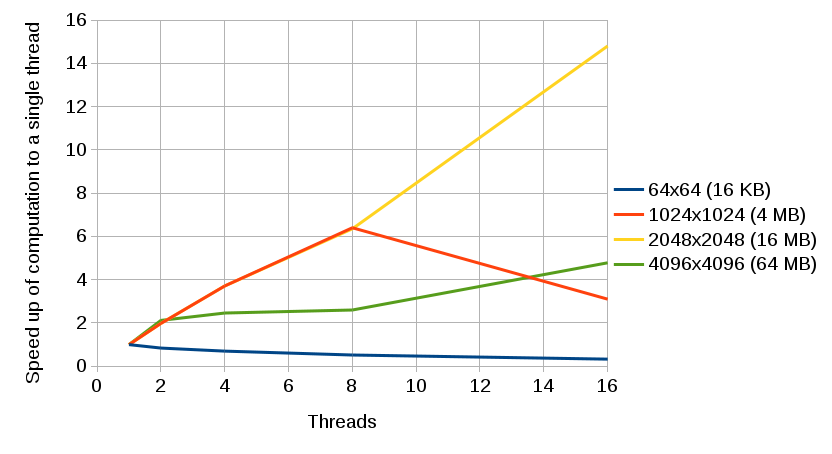
\includegraphics[width=1\linewidth]{fig/matvec_scaling.png}
    \caption{Scale computation to more threads (CPU).}
    \label{fig:graph_matvec_2048_scaling}
\end{figure} 

So 1 CPU computed the result the fastest on 8 threads. Specifically in 0.135 seconds reaching performance 91\,gFLOPS (29\% of theoretical performance). Two CPUs achieved performance 173\,gFLOPS (28\%). The L1 and L2 miss rates is relatively balanced in comparison with results depicted in the Table \ref{tab:table_matvec_parallel_64} (fake memory sharing was eliminated by large matrix size). Figure \ref{fig:graph_matvec_2048_scaling} also shows that the most \uv{beautiful} scaling was reached with the matrix size 2048*2048. There is sufficient amount of data for all threads while data are still fitted in the L3 cache. Now that the algorithm is optimized sufficiently, we can move to the Intel Xeon Phi coprocessor.

%%%%%%%%%%%%%%%%%%%%
\subsection{Matvec on the Xeon Phi coprocessor}
The First step in transferring our application to the MIC will be a very simple adjustment of the \texttt{Makefile}. We add the \texttt{-mmic} parameter to compiler flags (\texttt{CXXFLAGS+='-mmic'}). This will make the compiler generate code for the MIC. We also have to remove the \texttt{-xavx} options since it is not supported by the MIC. Let's compile and run our program.

\bigskip
\begin{lstlisting}[language=bash, caption=Compilation and execution a native aplication for Xeon Phi., captionpos=b, label=code_compile_execute]
[host]$ cd nbody/omp-parallel-mic
[host]$ make
[host]$ ssh mic0
[mic0]$ cd nbody/omp-parallel-mic
[mic0]$ export OMP_NUM_THREADS=1 # later e.g. 120, 180, 240
[mic0]$ # following line - direcotory with MIC shared libraries
[mic0]$ export LD_LIBRARY_PATH=/path/to/lib/mic:$LD_LIBRARY_PATH
[mic0]$ ./matvec
\end{lstlisting}
\bigskip

Let's compare single thread performance of application (naive implementation on CPU, dynamic and aligned version on CPU \& MIC) at first. We can see great difference between naive (no optimizations) implementation and optimized version in Figure \ref{fig:graph_matvec_comparasion_1thread} (more than 20 times faster). Figure \ref{fig:graph_matvec_comparasion_1thread} also shows that MIC has much worse results than CPU when we using only 1 thread (MIC is more than 10 times slower). It is mainly due to low core frequency and 2 cycles instruction decoding described in the Section \ref{sec:basic_info}.  

\begin{figure}[htbp]
    \centering
    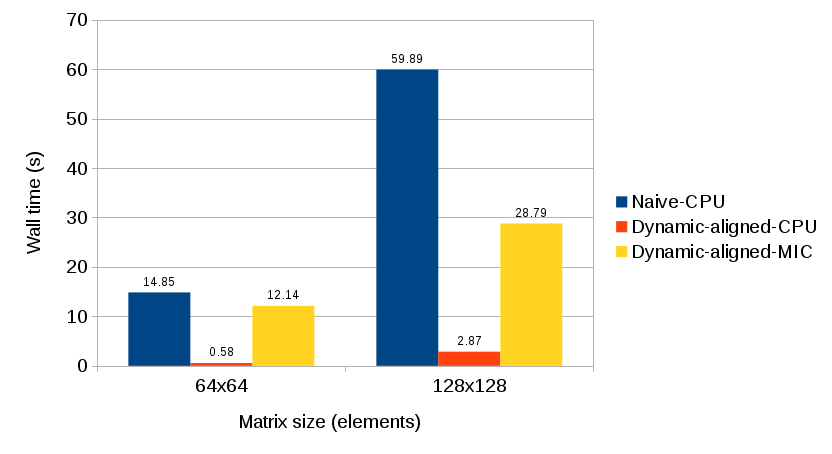
\includegraphics[width=1\linewidth]{fig/matvec_comparasion_1thread.png}
    \caption{Single thread comparison (CPU/MIC).}
    \label{fig:graph_matvec_comparasion_1thread}
\end{figure}

\par The MIC offers us significantly more hardware threads than the CPU. Therefore, we can start experimenting and execute the program using 1, 2, 4, 8, 16, 32, 60, 120, 180 and 240 threads. Figure \ref{fig:graph_matvec_2048_scaling_mic} and Table \ref{tab:table_matvec_2048_scaling_mic} contain results of the measurements for the matrix 2048*2048 elements (16\,MB) and 1000 repetitions. As we can see from the Figure \ref{fig:graph_matvec_2048_scaling_mic} and Table \ref{tab:table_matvec_2048_scaling_mic}, the MIC needs much more threads to achieve satisfactory results. But the dependency of a speed up (on threads number) and process of scaling can be clearly seen. More data means better workload of the threads and we can see more \uv{beautiful} scaling. 

\par However, at the end we achieved only slightly better result than on the processor. The coprocessor calculated the result on 240 threads in 1.127 seconds, which almost equal with 1.135 second that achieved processor (8 threads). Two CPUs are in this case much better than MIC (almost 2 times).

\begin{table}[ht]
\catcode`\-=12
\begin{center}
\begin{tabular}{| l | r |} \hline
\textbf{Threads} & \textbf{Wall Time (s)}\\ \hline
1 & 4.042\\ \hline
2 & 3.824\\ \hline
4 & 3.841\\ \hline
8 & 1.983\\ \hline
16 & 1.098\\ \hline
30 & 0.599\\ \hline
60 & 0.360\\ \hline
120 & 0.246\\ \hline
180 & 0.164\\ \hline
240 & 0.127\\ \hline
\end{tabular}
\caption{Performance measurement of omp parallel version, matrix size 2048*2048 elements (16\,MB, MIC).}
\label{tab:table_matvec_2048_scaling_mic}
\end{center}
\end{table}

\begin{figure}[htbp]
    \centering
    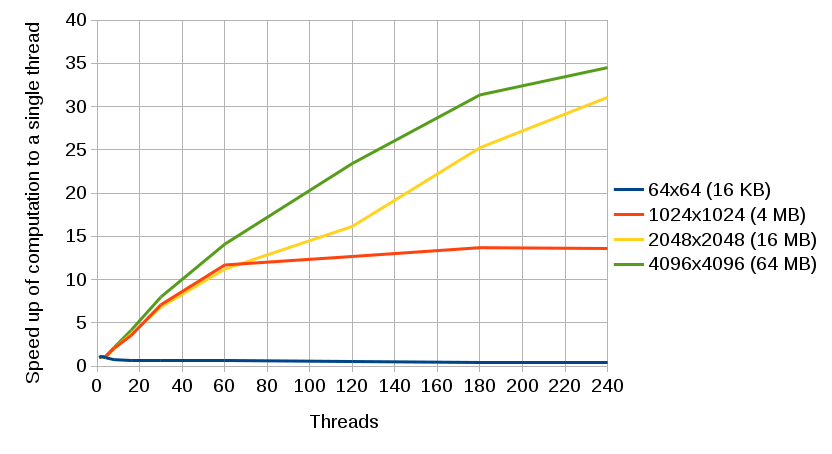
\includegraphics[width=1\linewidth]{fig/matvec_scaling_mic.png}
    \caption{Scale computation to more threads (MIC).}
    \label{fig:graph_matvec_2048_scaling_mic}
\end{figure} 

\par Therefore, we must even try to increase the matrix size (lot of threads == overhead) and compare the results. Graph \ref{fig:graph_matvec_xeon_vs_phi} describes comparison of CPU and MIC performance. We can see that with matrix size 8192*8192 is performance of the MIC more than 5 times higher than performance of the CPU (and 3 times higher than 2 CPUs). In this case we achieved performance about 130\,gFLOPS on the MIC\,--\,6.5\% of theoretical performance (1 CPU\,--\,8\% and 2 CPU\,--\,6.7\%). 

\begin{figure}[htbp]
    \centering
    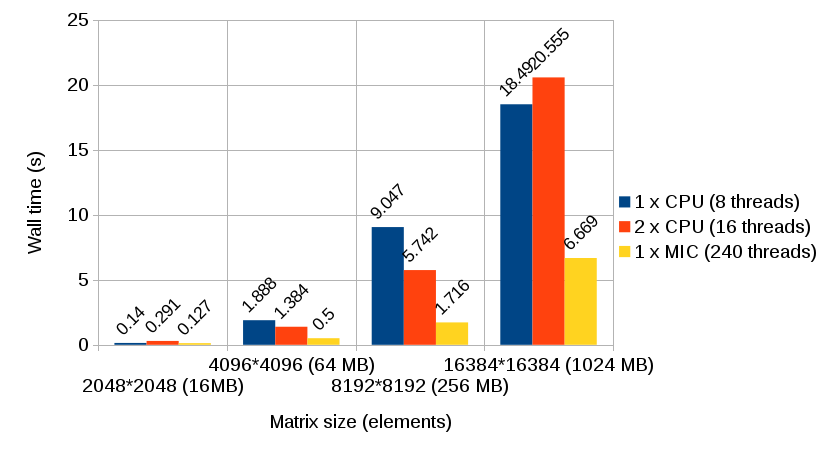
\includegraphics[width=1\linewidth]{fig/matvec_xeon_vs_phi.png}
    \caption{Matvec comparison CPU vs. MIC.}
    \label{fig:graph_matvec_xeon_vs_phi}
\end{figure} 

Of course we have not used all available optimization possibilities (6.5\% of theoretical performance is not very much), but for demonstration purposes this level of optimization is sufficient. It would definitely be suitable to compute multiplication for data block the approximate size of cache memory (cache blocking), but we will deal with this in the N-Body benchmark. Implementation of this task is nice mainly as \uv{tutorial}, in real situations is better to use highly optimized routines, e.g. from Intel MKL. Source files of this step can be found in the directory \texttt{matvec/omp-parallel-mic}.

%%%%%%%%%%%%%%%%%%%%%%%%%%%%%%%%%%%%%%%%
\section{Multiplication of two matrixes (matmul)}
From the matrix vector multiplication we now move to multiplication of two matrixes. This time we won't implement the algorithm itself. We will experiment with optimized routine from the MKL\,--\,DGEMM. The DGEMM (in our case \texttt{cblas\_dgemm}) function compute matrix multiplication for double precision data. Since this function is part of the Intel MKL library, it is highly optimized for the CPU as well as the MIC. Except for this it can highly utilize the potential of the machine. We can therefore directly test speed up of the MIC in comparison to the CPU (or 2 CPUs). Moreover, we can demonstrate the use of the Auto Offload mode here.

\par Let's start with the matrix of the size 1024*1024 (we will gradually double this size). To see results of this experiment look at Figure \ref{fig:graph_matmul_xeon_vs_phi}.

\begin{figure}[htbp]
    \centering
    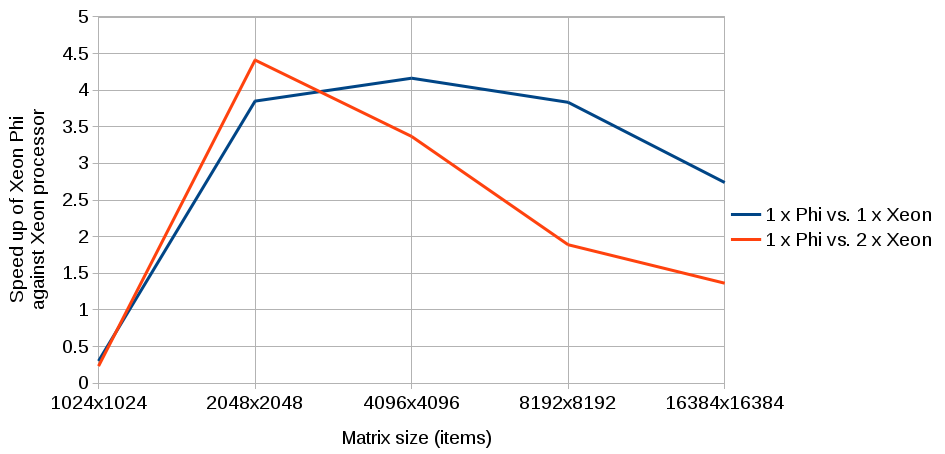
\includegraphics[width=1\linewidth]{fig/matmul_xeon_vs_phi.png}
    \caption{Speed up of the MIC against the CPU in the matrix multiplication (matmul).}
    \label{fig:graph_matmul_xeon_vs_phi}
\end{figure} 

\par Unfortunately, we weren't able to measure performance of DGEMM by PAPI (only wall time). On the other hand, Intel published their SGEMM/DGEMM benchmark \footnote{SGEMM/DGEMM benchmark by Intel:\\ \url{http://www.intel.com/content/www/us/en/benchmarks/server/xeon-phi/xeon-phi-sgemm-dgemm.html}} and we can compare our results. Intel achieved performance 837\,gFLOPS (on the MIC same as our one) which is 83\% of theoretical performance. Two CPUs (16 threads) produced performance 548\,gFLOPS which is about 1.5 time smaller than the performance of the MIC. For the matrix size 16384*16384 are our results very similar (Intel used similar matrix size). The MIC is much faster in comparison with 1 CPU (4 times for matrix 4096*4096). It means that using of MIC can has a sense.

\par If we want to use the Automatic Offload (AO), we have to compile the code for the CPU (without \texttt{-mmic}), set the environment variable \texttt{export MKL\_MIC\_ENABLE=1} and execute the program. If we want to check whether offload was performed, we set the environment variable \texttt{export OFFLOAD\_REPORT=2}. If we want to set the number of coprocessor threads, we set \texttt{export MIC\_ENV\_PREFIX=MIC; export MIC\_OMP\_NUM\_THREADS=240}. When executing the program with various matrix sizes we discover that the AO takes place only after crossing a certain matrix size. This is caused by library runtime heuristics which allows AO only if it presumes that the computation on the MIC would has sense.

\par Automatic Offload can also be used for example with Python language, specifically with modules Numpy and Scipy. If we want to use AO with this modules, they will have to be linked with Intel MKL.

\par In this example we can simply experiment with \texttt{KMP\_AFFINITY}. Graph \ref{fig:matmul_affinity} shows differences of wall times when we are using \texttt{compact} or \texttt{scatter} threads affinity. As we can see, importance of threads affinity depends on matrix size (generally depends mainly on specific algorithm). Source code of examples associated with this section can be found in the \texttt{matmul/} directory.

\begin{figure}[htbp]
    \centering
    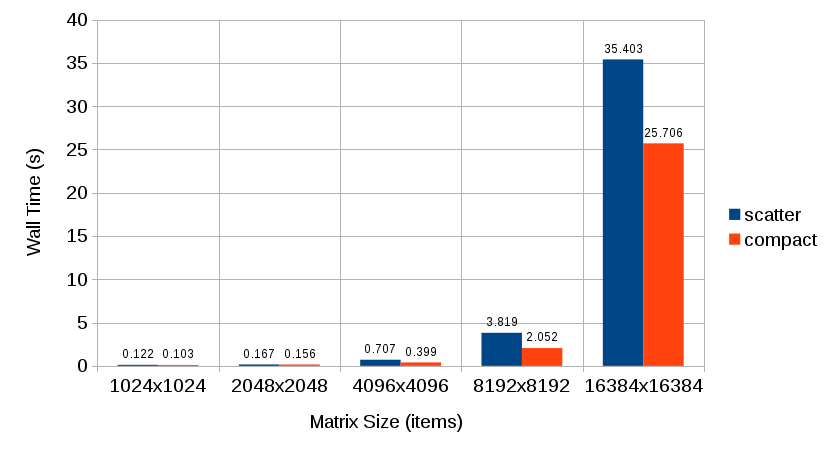
\includegraphics[width=1\linewidth]{fig/matmul_affinity_test.png}
    \caption{Comparison of the \texttt{compact} and the \texttt{scatter} threads affinity (matmul).}
    \label{fig:matmul_affinity}
\end{figure} 

%%%%%%%%%%%%%%%%%%%%%%%%%%%%%%%%%%%%%%%%
\section{N-Body Simulation}

%%%%%%%%%%%%%%%%%%%%
\subsection{Introduction of the benchmark}
N-Body is some physical simulation strongly associated with HPC. There are lot of benchmarks (with some modifications) dealing with this problem. It is a more complex task incorporating significantly more computations (not only MAD like matvec). It will be a computation of mutual force influence of bodies and its optimization. Each body has a certain weight, speed and position in space. Gravitational forces of other bodies affect the specific body. Their forces have various directions and their resultant causes a change in body speed. At first it is necessary to compute the force affecting every body. It is given by vector sum of partial forces caused by gravitational effect of other bodies. We compute the force between 2 bodies by equation \ref{eq:eq_force}.

\begin{equation}
F = \frac{G * m_1 * m_2}{R^2}
\label{eq:eq_force}
\end{equation}

\texttt{F} is force between 2 bodies, \texttt{G} is gravitational constant, $m_1, m_2$ are weights of bodies, \texttt{R} is distance between bodies. Having this force we can calculate the acceleration of body by equation \ref{eq:eq_acceleration}.

\begin{equation}
a^{(i+1)} = \frac{\sum{F^{i+1}_n}}{m}
\label{eq:eq_acceleration}
\end{equation}

Consequently we can calculate new velocity of the body by equation \ref{eq:eq_velicity}

\begin{equation}
v^{(i+1)} = v^i + a^{(i+1)} * \Delta T
\label{eq:eq_velicity}
\end{equation}

The last equation \ref{eq:eq_position} is used to calculate a new position of the body.

\begin{equation}
r^{(i+1)} = r^i + v^{(i+1)} * \Delta T
\label{eq:eq_position}
\end{equation}

To summarize, in each step we compute forces among individual bodies, changes of the speed and positions. The simulation of N particles movement in STEPS steps can be describe by Pseudo code \ref{code_nbody_algorithm}.

\bigskip
\begin{lstlisting}[caption=Pseudo code of the N-Body algorithm., captionpos=b, label=code_nbody_algorithm]
// each step of simulation
for(step = 0; step < steps; step++)
{
    // iterate through all bodies
    for(i = 0; i < N; i++)
    {
        // calculate force between bodies
        for(j = 0; j < N; j++)
        {
            if(particle[i] != particle[j])
                F = calculate_force(particle[i], particle[j]);
        }
        // calculate acceleration
        ACC = calculate_acc(particle[i], F);
        // calculate velocity
        VEL = calculate_vel(particle[i], ACC);
        // calculate position
        POS = calculate_pos(particle[i], VEL);
    }   
}
\end{lstlisting}
\bigskip

%%%%%%%%%%%%%%%%%%%%
\subsection{Naive implementation}
Let's start with a simple implementation to validate the code. During implementation we can proceed according to the relations stated above and the Pseudo code \ref{code_nbody_algorithm}. Like in the matvec benchmark the application was implemented and optimized for the CPU at first. After compiling the program through appended Makefile and subsequent execution, we achieved results shown in Table \ref{tab:table_nbody_naive}. As we can see the results are not satisfactory, mainly due to very small number of vector operations.

\begin{table}[ht]
\catcode`\-=12
\begin{center}
\begin{tabular}{| l | r | r |} \hline
\textbf{Number of bodies} & 1000 (27.3\,KB) & 10000 (273\,KB)\\ \hline
\textbf{Wall Time (s)} & 16.000 & 1600.270\\ \hline
\textbf{Scalar FP Ops (mFLOPS)} & 1499.51 & 1500.45\\ \hline
\textbf{Vector FP Ops (mFLOPS)} & 250.75 (0.65\%) & 250.79 (0.65\%)\\ \hline
\textbf{L1 miss} & 0\% & 10\%\\ \hline
\textbf{L2 miss} & 1\% & 2\%\\ \hline
\end{tabular}
\caption{Performance measurement of the naive implementation (CPU).}
\label{tab:table_nbody_naive}
\end{center}
\end{table}

After confirming the accuracy of the computation, this version of the program was taken as reference for checking the correctness of the computation and optimization of the algorithm. At first glance the code is far from optimized ones, therefore several steps for optimization have to be taken. We will proceed just like with matrix vector multiplication. This implementation can be found in the \texttt{nbody/naive} directory.

%%%%%%%%%%%%%%%%%%%%
\subsection{Algorithm enhancement, automatic optimizations}
So far our code contains badly designed algorithm especially with respect to the structure of loops, jumps in loops and data storage in memory. First step is the removal branches from the loop. This branch is to ignore the identical particles (this avoiding division by zero). The condition was removed by adding very small constant to the distance between the particles. The constant has such a small value that its consequence on accuracy of the computation is negligible.

\par Further, it is necessary to adjust data layout in memory. For clarity it is good to cover individual particle attributes into a structure. As we explained in the theoretical part, there is a big difference between array of structures or structure of arrays where SoA is said to be more SIMD-friendly. Again we choose dynamic allocation and data alignment to 64\,Bytes. After the modification of the algorithm we get significantly better results (see Table\ref{tab:table_nbody_enhancement}).

\begin{table}[ht]
\catcode`\-=12
\begin{center}
\begin{tabular}{| l | r | r |} \hline
\textbf{Number of bodies} & 1000 (27.3\,KB) & 10000 (273\,KB)\\ \hline
\textbf{Wall Time (s)} & 1.110 & 107.120\\ \hline
\textbf{Scalar FP Operations (mFLOPS)} & 17.85 & 1.84\\ \hline
\textbf{Vector FP Operations (mFLOPS)} & 26165.70 (68\%) & 27076.60 (70\%)\\ \hline
\textbf{L1 miss} & 0\% & 22\%\\ \hline
\textbf{L2 miss} & 2\% & 2\%\\ \hline
\end{tabular}
\caption{Performance measurement of a better implementation (still single thread), automatic optimizations (CPU).}
\label{tab:table_nbody_enhancement}
\end{center}
\end{table}

The results speak for themselves; the computation time shrank almost 15 times, not to mention the number of vector computations. It's worth mentioning that there is not a single compiler directive, it is exclusively the code structure enhancement, better data layout and automatic optimization of the compiler. It needs to be said that the application is still running only on 1 thread. Performance 27\,gFLOPS is very good result, it is 70\% of theoretical performance. Source codes can be found in the directory \texttt{nbody/non-jump-auto-opt}.

%%%%%%%%%%%%%%%%%%%%
\subsection{Parallel processing on thread level}
\label{sec:body_omp}
When looking at a force computation, we can see that a loop is still complicated. It is possible to exempt computation of acceleration (and particle speed) from this loop. We must store resultant force (for each particle) to array, which we will add to the structure of the particle system. Thus we can compute acceleration and new speed in an individual loop; we compute the new particle position in the same way. These shorter and simpler loops can be vectorized better. On the other hand, structure of particles system now contains 13 arrays (not 7 as in previous case). This means that we will work with 50.7\,KB (1000 bodies) and 507\,KB (10000 bodies) of data (we use single precision).

\par Let's add the \texttt{omp parallel for} directive above loops which can be executed in parallel. In our case it is the loops for initiation of force, computation of force, computation of acceleration, computation of speed and computation of position. Further, we add the directive \texttt{simd} above loops which can be vectorized (the most nested loops). At this point we will try to run improved program on a single thread and compare results. See Table \ref{tab:table_nbody_omp_1thread} for complete results. Note that number of scalar operations is very small.

\begin{table}[ht]
\catcode`\-=12
\begin{center}
\begin{tabular}{| l | r | r |} \hline
\textbf{Number of bodies} & 1000 (50.7\,KB) & 10000 (507\,KB)\\ \hline
\textbf{Wall Time (s)} & 1.022 & 104.105\\ \hline
\textbf{Scalar FP Operations (mFLOPS)} & 0.14 & 0.07\\ \hline
\textbf{Vector FP Operations (mFLOPS)} & 28494.30 & 28020.80\\ \hline
\textbf{L1 miss} & 1\% & 30\%\\ \hline
\textbf{L2 miss} & 1\% & 1\%\\ \hline
\end{tabular}
\caption{Performance measurement of the omp version, single thread only (CPU).}
\label{tab:table_nbody_omp_1thread}
\end{center}
\end{table}

\par It's good to advise the compiler that the data in memory is aligned. However, due to a large number of threads the alignment breaks down and the program crashes might occur. Therefore, for simplicity we will execute the program for such number of particles for which data will be still aligned even after particles distribution among all threads. Now we will run the computation for 10000 particles and 1000 steps subsequently on 1, 2, 4, 8 and 16 threads. The results of the measurements are listed in Table \ref{tab:table_nbody_scaling} and Figure \ref{fig:graph_nbody_scaling}. 

\begin{table}[ht]
\catcode`\-=12
\begin{center}
\begin{tabular}{| l | r | r | r | r |} \hline
\textbf{Threads} & \textbf{Wall Time (s)} & \textbf{Vector FP Ops (mFLOPS)} & \textbf{L1 miss} & \textbf{L2 miss}\\ \hline
1 & 103.937 & 28063.3 & 30\% & 1\%\\ \hline
2 & 552.254 & 55831.3 & 31\% & 1\%\\ \hline
4 & 26.164 & 111453.0 & 31\% & 1\%\\ \hline
8 & 13.745 & 212304.0 & 31\% & 2\%\\ \hline
16 & 0.532 & 393308.0 & 30\% & 3\%\\ \hline
\end{tabular}
\caption{Performance measurement of the omp parallel version, 10000 bodies, scaling (CPU).}
\label{tab:table_nbody_scaling}
\end{center}
\end{table}

\begin{figure}[htbp]
    \centering
    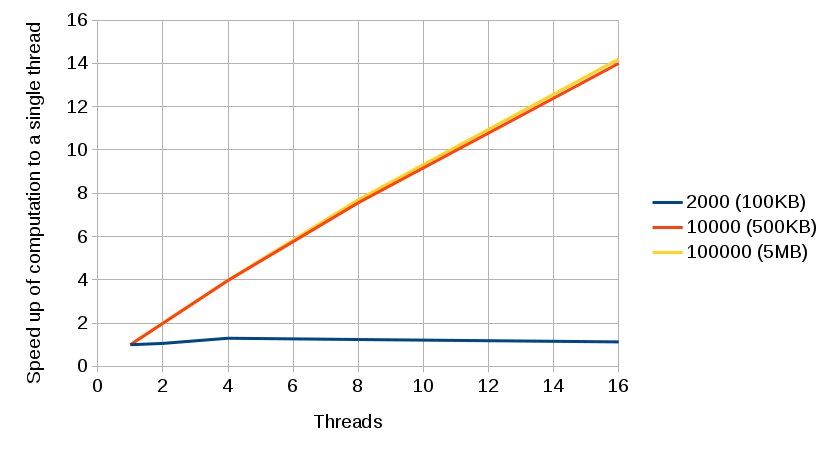
\includegraphics[width=1\linewidth]{fig/nbody_scaling.png}
    \caption{Scale the computation to a more threads (CPU).}
    \label{fig:graph_nbody_scaling}
\end{figure} 

Figure \ref{fig:graph_nbody_scaling} clearly shows dependency of computation time on the number of threads. Computation took 13.745 seconds on 8 threads while we achieved performance more than 210\,gFLOPS (68\% of theoretical). Two CPUs provide performance 390 gFLOPS (63\%). When we work with only 2000 particles, the  performance is almost same for single thread and for more threads (2, 4, 8, 16). It can be caused by bad workload of each thread. If we exceed a certain threshold (number of bodies), scaling is much better (see Figure \ref{fig:graph_nbody_scaling}). Source codes can be found in the directory \texttt{nbody/omp-parallel}.

%%%%%%%%%%%%%%%%%%%%
\subsection{N-Body on the Xeon Phi coprocessor}
First, we will compare single tread programs. It will be naive implementation on CPU and previous implementation (Section \ref{sec:body_omp}) on CPU \& MIC. We can see (Figure \ref{fig:graph_nbody_1thread}) similar results to matvec (Figure \ref{fig:graph_matvec_comparasion_1thread}). Single thread application running on MIC has about 5 time worse results than on the CPU.

\begin{figure}[htbp]
    \centering
    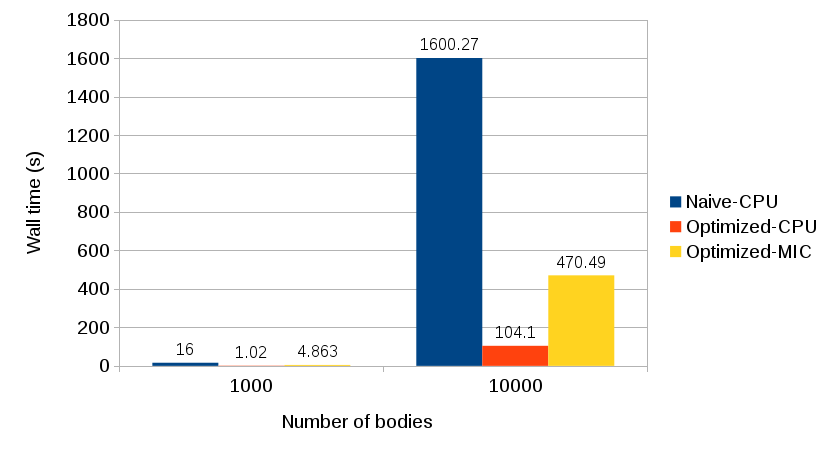
\includegraphics[width=1\linewidth]{fig/nbody_compare_1thread.png}
    \caption{Single thread comparison (CPU/MIC).}
    \label{fig:graph_nbody_1thread}
\end{figure} 

\par The next step will be the program execution (10000 bodies and 1000 repetitions) on the MIC, while using 1, 2, 4, 8, 16, 32, 60, 120, 180 and 240 threads. Figure \ref{fig:graph_nbody_scaling_mic} and Table \ref{tab:table_nbody_scaling_mic} depicts the course of the application scaling (on the MIC). The computation time when using 240 threads was 3.4 times smaller than on the CPU. It means that performance on 240 threads provide more than \textbf{725\,gFLOPS} (36\% of theoretical performance). On the other hand, single thread computation took as long as 471 seconds, which is about 4 times more than when using 1 thread on the CPU. These results speak for themselves. The key to high performance on the MIC is without a doubt using a large number of threads. We can also see course of scaling for other number of bodies. E.g. 2000 particles have slower scaling course (small threads workload) than greater numbers of bodies. 

\par However, we are not yet done with optimization, there are still several possibilities, through which we can better utilize the potential of the MIC. The source codes are available in the directory \texttt{nbody/omp-parallel-mic}.

\begin{table}[ht]
\catcode`\-=12
\begin{center}
\begin{tabular}{| l | r |} \hline
\textbf{Threads} & \textbf{Wall Time (s)}\\ \hline
1 & 471.662\\ \hline
2 & 267.336\\ \hline
4 & 226.572\\ \hline
8 & 108.587\\ \hline
16 & 54.360\\ \hline
30 & 29.479\\ \hline
60 & 15.161\\ \hline
120 & 7.908\\ \hline
180 & 5.253\\ \hline
240 & 4.017\\ \hline
\end{tabular}
\caption{Performance measurement of the omp parallel version, 10000 bodies and 1000 runs (MIC).}
\label{tab:table_nbody_scaling_mic}
\end{center}
\end{table}

\begin{figure}[htbp]
    \centering
    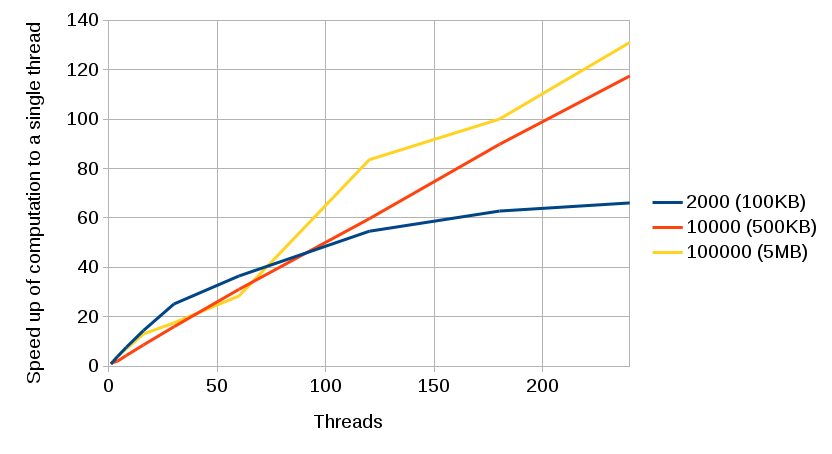
\includegraphics[width=1\linewidth]{fig/nbody_scaling_mic.png}
    \caption{Scale computation to a more threads (MIC).}
    \label{fig:graph_nbody_scaling_mic}
\end{figure} 

%%%%%%%%%%%%%%%%%%%%
\subsection{Cache blocking}
The Xeon Phi coprocessor offers us very quick cache memories. The next step of optimization will be the effort to exploit cache memories as best as possible. For this step we will use the famous method\,--\,cache blocking. This method is based on splitting a large number of data into smaller blocks, usually blocks of the cache size. The principle is using the data stored in cache as many times as it's possible before moving them again to the main memory. This data reusable (from the cache memory) eliminates the number of accesses to the main memory, thus the CPU/MIC doesn't have to wait so long for the data. The process for loop tiling may look like:

\bigskip
\begin{lstlisting}[caption=Pseudo code of the cache-blocking., captionpos=b, label=code_nbody_algorithm]
// simple iterating through array
for(i = 0; i < N; i++)
{
    A[i] = do_something();
}

// cache-blocking
for(i = 0; i < N; i += BLOCK)
{
    for(b = j; b < min(N, j + BLOCK); b++)
    {
        A[b] = do_something();
    }
}
\end{lstlisting}
\bigskip

Setting the correct block size for processing doesn't have to be decisive. It depends on the cache size (there is a difference if we want to keep the data in L1 or L2 cache), type of algorithm, etc. We must experiment with the block size, we can start e.g. with the size 1/2 of L1 cache. We subsequently increase the block size and observe the acceleration/slowdown of computation. Now, we will run simulation for much more particles because we must have data bigger than all caches (e.g. 1105920 particles). Figure \ref{fig:graph_nbody_blocking} describes differences among wall times of programs with the various block sizes. We can see that we have not achieved satisfactory results with any block size. It can be caused by strong hardware and software prefetching or some other hardware and compiler optimizations. Source code can be found in the directory \texttt{nbody/cache-block-mic}.

\begin{figure}[htbp]
    \centering
    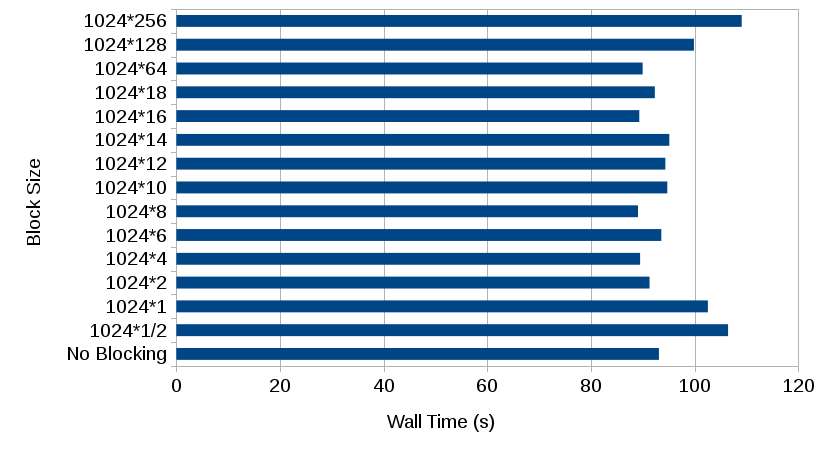
\includegraphics[width=1\linewidth]{fig/nbody_blocking.png}
    \caption{Cache blocking, various block sizes (MIC).}
    \label{fig:graph_nbody_blocking}
\end{figure} 

%%%%%%%%%%%%%%%%%%%%
\subsection{Offload mode}
So far we have been dealing with programming of native applications for Xeon Phi. As we said at the beginning, Xeon Phi is not capable to process I/O operation as fast as the CPU. Before beginning the computation, our program reads large amount of data from the file. After completing the computation writes the same amount of data into the file. Data reading time from file on the MIC is several times higher than on the CPU; therefore we will try to use the offload mode. The program will be run on the host system. Host reads the data and sends it to the MIC. After that, the MIC runs a simulation and sends the data back to the host system (CPU subsequently writes them in a file). In this case, the implementation will be more difficult than with the native mode. This is complicated by the fact that it is not possible to copy other than simple data types to the MIC (it cannot be a structure of pointers). Before copying the data to the MIC we have to perform manual decomposition of pointer structure to individual arrays, which we copy to the MIC and store back to the structure. We add required offload directives and compile the program. This time the program will be compiled for the host system, i.e. without the \texttt{-mmic} option. 

\par The comparison of the individual program sections (MIC native vs. CPU + offload to MIC) is depicted in Figure \ref{fig:graph_nbody_offload_vs_native}. When we read/write 1105920 bodies from the file via \texttt{fprintf} function, we achieved much worse results on the MIC than on the CPU. The CPU handles I/O (single thread) operation so much better. It is more efficient to use some king of buffers and read/write bigger chunks of data, less times (binary read/write is also faster than \texttt{fprintf}). Source codes for the offload mode are available in the directory \texttt{nbody/offload}.

\begin{figure}[htbp]
    \centering
    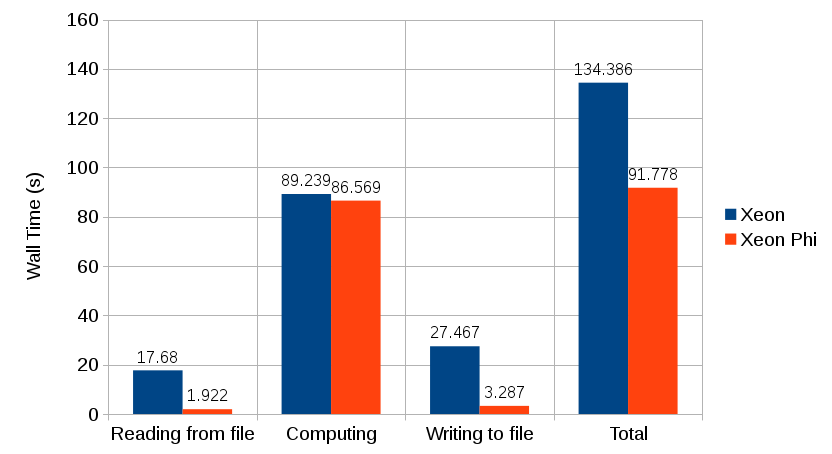
\includegraphics[width=1\linewidth]{fig/nbody_offload_vs_native.png}
    \caption{Comparasion of the native and the offload mode (N-Body), 1105920 bodies.}
    \label{fig:graph_nbody_offload_vs_native}
\end{figure} 

%%%%%%%%%%%%%%%%%%%%%%%%%%%%%%%%%%%%%%%%
\section{K-Wave}
K-Wave is an open source toolbox for MATLAB, dealing with the simulation of acoustic waves propagation in 1D, 2D and 3D. It comprises of thousands lines of source code (C++ language) optimized for CPU using OpenMP. So this time we will not be creating the code itself, we will try to port the application to the MIC, measure performance, compare with CPU and eventually optimize. We will not be dealing with the internal structure of the program; we will only sum up the most basic information.

\par The program itself is composed of a large number of demanding computations. The combination of this computations creates the simulation itself. Simulation uses own kernels, but in majority of cases functions from the MKL library. It uses especially FFT functions forming the biggest part of the simulation. For data load/store operations it uses the HDF5 library, for data compression the ZLIB library.

\par For the program compilation it's necessary to prepare the HDF5 and ZLIB libraries for the MIC (non-standard libraries). Procedure of libraries compilation for the MIC will be described in the Section \ref{sec:crosscompilation}.

\par After successful compilation, we can move to the performance testing on the MIC. Immediately after starting the program we discover that the computation time on the MIC is approx. two times longer than on the CPU. With a complicated project like this it is more difficult to discover the reasons for the low performance. However, the Intel VTune Amplifier (profiling tool) serves us very good for this purpose. After the application profiling we discover that a big part of the computation time is taken especially by the FFT functions from the MKL library. This fact is not very heartwarming, because we are not able to affect the performance of these functions. The profiling results show that the FFT functions on the MIC takes longer time than on the CPU.

\par We have therefore decided to measure the performance of the FFT functions (on the CPU \& MIC) by means of simple benchmarks. On 1 CPU we achieved performance of circa 70\,gFLOPS (8 threads), on 2 CPUs 115\,gFLOPS (depending on processed data size, etc.). The MIC achieved in majority of cases worse results or hardly reached the performance of the CPUs.

\par Searching the web we can find other benchmarks related to FFT and Intel Xeon Phi, where results similar to ours were achieved. The performance of Xeon Phi also reached around 100\,gFLOPS. However, we were not able to solve this problem. It is possible that the new MKL version will bring also a better FFT performance on the MIC.

%%%%%%%%%%%%%%%%%%%%%%%%%%%%%%%%%%%%%%%%
\section{Cross-compilation of existing libraries, modules, programs}
\label{sec:crosscompilation}
Very interesting part of this work was the effort of porting various libraries, modules or programs to the MIC. These included e.g. HDF5 library (data model, file format for data storing), ZLIB or BZIP2 libraries (data compression). A more complex problem was the cross-compilation of the Python interpreter and its Numpy, Scipy or Ctypes modules. The Numpy and Scipy modules are widely used, especially in HPC sphere. They contain a large number of data types and highly optimized routines. Furthermore, these modules can be linked directly with the MKL library. The effort for native running of stated libraries and modules on the MIC was successful (from the functional point of view). From the performance point of view (e.g. Python language interpreter) it was worse. As already mentioned, low performance of the Xeon Phi cores does not allow \uv{quick} running of the programs using only 1 thread. The Python interpreter executes the code sequentially (with the exception of optimized functions calls), thus using only 1 thread.

\par Regarding the cross-compilation of existing programs (for the MIC), it can be simple or very difficult. Standard compilation and installation takes place usually in the following steps:

\begin{enumerate}
\item{Execution of a configuration script (\texttt{./configure})} 
\item{Compilation of a source files (\texttt{make})}
\item{Installation (\texttt{make install})}
\end{enumerate}

Various parameters can be given to the configuration script affecting the compilation. So if we compile for the MIC, it is necessary to set the correct compiler options. E.g. we have to state that we want to use the Intel compiler (\texttt{CC=icc}) and generate the binary for the MIC (\texttt{CFLAGS=-mmic}). It's not always such easy; sometimes it is necessary to manually adjust the Makefiles, configuration scripts, etc. The directory \texttt{cross-compilation} contains some procedures of cross-compilation (ZLIB, BZIP2 or HDF5 libraries). These procedures are only \uv{demo}, for other versions of the libraries it might be necessary to do other adjustments.

%%%%%%%%%%%%%%%%%%%%%%%%%%%%%%%%%%%%%%%%
\section{Extraction of I-vector}
Python running natively on the MIC was designed for research group at the FIT VUT focused on speech processing. It was so called the Extraction of I-vector, which is quite a significant part of speech processing. The application was created in the Python language and used optimized routines calls from Intel MKL.

\par As already mentioned, the performance of the Python interpreter on the MIC was not satisfactory. Sections of the code based on calling the MKL functions displayed signs of acceleration. But the code executed sequentially (1 thread) literally buried the entire program. For comparison the program wall time on the MIC was approx. 20 times higher than on the CPU. The biggest part of the application wall time was reading the data from file (expected behavior). But even with computations themselves the coprocessor didn't fair better than the CPU. Figure \ref{fig:ivector_comparasion} depicts comparison (wall times) of individual parts of I-vector extractions (1 x CPU vs. 1 x MIC).

\begin{figure}[htb]
    \centering
    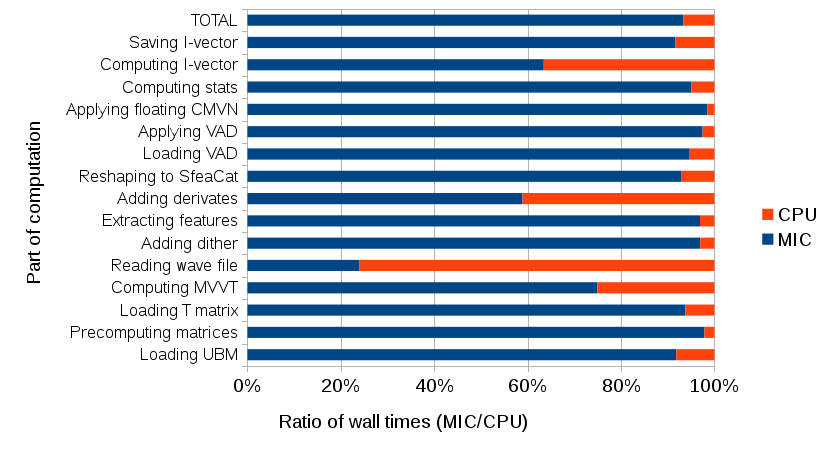
\includegraphics[width=1\linewidth]{fig/ivector_comparasion.png}
    \caption{I-vector extraction, comparasion of individual parts, CPU vs. MIC.}
    \label{fig:ivector_comparasion}
\end{figure}

%%%%%%%%%%%%%%%%%%%%%%%%%%%%%%%%%%%%%%%%%%%%%%%%%%%%%%%%%%%%%%%%%%%%%%%%%%%%%%%
\chapter{Conclusion}
This thesis deals with the implementation and optimization of a high performance algorithms on the Intel Xeon Phi. For demonstration purposes, simple benchmarks have been implemented, from which we moved on to more complex ones. To gain experience with the MIC, the matrix vector multiplication has been chosen. The benchmark has been implemented for the CPU reaching the performance 90\,gFLOPS (29\% of the theoretical performance) at the first. This task reached performance about 130\,gFLOPS on the MIC (6.5\%). Acceleration in this case isn't significant, but in some cases (big matrix) a speed up of the MIC can be more than 4-fold. A similar algorithm was the matrix multiplication (we used optimized function from the Intel MKL). The MIC was doing quite well; with sufficient data it reached more then 4-fold acceleration (compared with the CPU). However, due to problem with the PAPI we were unable to measure the maximum performance (gFLOPS).

\par Algorithm reaching significantly higher performance on the CPU and the MIC was the N-body simulation. The quickest version of the algorithm produced performance 210\,gFLOPS (68\%\,--\,1 x CPU), 390\,gFLOPS (63\%\,--\,2 x CPU) and 725\,gFLOPS (36\%\,--\,1 x MIC).
The next step in our work was the porting of MATLAB module k-Wave to the Xeon Phi. The effort to accelerate the computations by using Xeon Phi was unsuccessful due to strange behavior of the FFT functions (from the MKL library). These functions did not display signs of a speed up on the MIC. It was quite the opposite, in many cases they were slower. The problem might be solved in the newer version of Intel MKL.

\par Conclusion of the thesis is focused on cross-compilation of existing libraries, modules and programs. It deals e.g. with libraries for work with files (HDF5, ZLIB, SZIP), interpreter of the Python (with Numpy and Scipy modules). Python running on the Xeon Phi should have been used for speech processing, specifically for the I-vector extraction. However, the Xeon Phi did not bring any speed up, quite the opposite, it brought a multiple slowdown.

\par All the experiments show that the Xeon Phi is definitely suitable only for highly parallel tasks regarding threads and SIMD instructions. It is not suitable for programs, which contain demanding computations processed sequentially (by using 1 thread or scalar operations). When combining parallel and sequential computations, it is suitable to use the offload mode or the CPU only.

\par I would like to continue in my work with Xeon Phi in the future, since a new supercomputer\,--\,Salomon (in Ostrava) will be soon ready for use. The Salamon will contains a large number of Xeon Phi coprocessors. The plan includes e.g. the use of several coprocessors for parallel solving of complex tasks.
%=========================================================================
